\documentclass[hidelinks]{article} % For LaTeX2e
\usepackage{iclr2016_conference,times}
\usepackage{hyperref}
\usepackage[section]{placeins}
\usepackage{url}
\usepackage{physics}
\usepackage{amsmath}
\usepackage{graphicx,import}
\usepackage[norelsize]{algorithm2e}


\title{The Incredible Shrinking Neural Network: Pruning to Operate in Constrained Memory Environments}

%\author{Nikolas Wolfe, Aditya Sharma, Lukas Drude \& Bhiksha Raj \\
%Language Technologies Institute\\
%Carnegie Mellon University\\
%Pittsburgh, PA 15213, USA \\
%\texttt{\{nwolfe, adityasharma, bhiksha\}@cmu.edu}\\
%\texttt{\{drude@nt.upb.de}\}
%}

\author{Nikolas Wolfe, Aditya Sharma, Bhiksha Raj\\
School of Computer Science\\
Carnegie Mellon University\\
Pittsburgh, PA 15213, USA \\
\texttt{\{nwolfe, bhiksha\}@cs.cmu.edu, {adityasharma}@cmu.edu}\\
}


% The \author macro works with any number of authors. There are two commands
% used to separate the names and addresses of multiple authors: \And and \AND.
%
% Using \And between authors leaves it to \LaTeX{} to determine where to break
% the lines. Using \AND forces a linebreak at that point. So, if \LaTeX{}
% puts 3 of 4 authors names on the first line, and the last on the second
% line, try using \AND instead of \And before the third author name.

\newcommand{\fix}{\marginpar{FIX}}
\newcommand{\new}{\marginpar{NEW}}
\newcommand{\Out}[2]{o_{#1}^{(#2)}}
\newcommand{\Target}[1]{t_{#1}}
\newcommand{\Input}[2]{x_{#1}^{(#2)}}
\newcommand{\Weight}[3]{w_{#1#2}^{(#3)}}
\newcommand{\Con}[3]{c_{#1#2}^{(#3)}}
\newcommand{\Etotal}{E_{\mathrm{total}}}

\setlength{\parindent}{0pt}

%\iclrfinalcopy % Uncomment for camera-ready version

\begin{document}


\maketitle

\begin{abstract}
We propose and investigate several methods for pruning neural networks to operate in constrained memory environments such as mobile or embedded devices. We first evaluate a simple pruning technique using first-order derivative approximations of the gradient of each neuron in an optimally trained network, and turning off those neurons which contribute least to the output of the network. We then show the limitations of this method by comparing its pruning decisions of this method against an exhaustive brute force approach to determining the change in error resulting from the removal of a given neuron. We attempt to improve on this using a second-order derivative approximation. We also explore the correlation between neurons in a trained network and attempt to improve our choice of candidate neurons for removal to account for faults that can occur from the removal of a single neuron at a time. We argue that this method of pruning allows for the optimal tradeoff in network size versus accuracy in order to operate within the memory constraints of a particular device or application environment. 
\end{abstract}
\section{Introduction}
Neural network pruning algorithms were first popularized by \cite{sietsma1988neural} as a mechanism to determine the proper size of a network required to solve a particular problem. To this day, network design and optimal pruning remain inherently difficult tasks. For problems which cannot be solved using linear threshold units alone, \cite{baum1989size} demonstrate there is no way to precisely determine the appropriate size of a neural network a priori given any random set of training instances. Using too few neurons inhibits learning, and so in practice it is common to attempt to over-parameterize networks initially using a large number of hidden units and weights. However, as \cite{chauvin1990generalization} writes, this approach can lead to over-fitting as the network's unnecessary free parameters start to latch on to idiosyncrasies in the training data. 


Pruning algorithms, as comprehensively surveyed by \cite{reed1993pruning}, are a useful set of heuristics designed to identify and remove network parameters which do not contribute significantly to the output of the network and potentially inhibit generalization performance. At the time of Reed's writing, reducing network size was also a practical concern, as smaller networks are preferable in situations where computational resources are scarce. In this paper we are particularly concerned with application domains in which space is limited and network size constraints must be imposed with minimal impact on performance.




\section{Related Work}
Neural network over-fitting is fundamentally a problem arising from the use of too many free parameters. Regardless of the number of weights used in a given network, as \cite{segee1991fault} assert, the representation of a learned function approximation is almost never evenly distributed over the hidden units, and the removal of any single hidden unit at random can actually result in a total network fault. \cite{mozer1989using} suggest that only a subset of the hidden units in a neural network actually latch on to the invariant or generalizing properties of the training inputs, and the rest learn to either mutually cancel each other out or begin over-fitting to the noise in the data. Determining which elements are unnecessary and removing them outright is therefore a well-founded approach to improving network generalization, and simultaneously provides a way to reduce their size in memory. 


The generalization performance of neural networks has been well studied, and apart from pruning algorithms many heuristics have been used to avoid overfitting, such as dropout (\cite{srivastava2014dropout}), maxout (\cite{goodfellow2013maxout}), and cascade correlation (\cite{fahlman1989cascade}), among others. However, these algorithms do not explicitly prioritize the reduction of network memory footprint as a part of their optimization criteria per se, (although in the opinion of the authors Fahlman's cascade correlation architecture holds great promise in this regard.) Computer memory size and processing capabilities have improved so much since the introduction of pruning algorithms in the late 1980s that space complexity has become a relatively negligible concern. The proliferation of cloud-based computing services has furthermore enabled mobile and embedded devices to leverage the power of massive data and computing centers remotely. In this domain, however, it is also reasonable to suggest that certain performance-critical applications running on low-resource devices could benefit from the ability to use neural networks locally. 

At present there are few (if any) mechanisms specifically designed to shrink neural networks down in order to meet an externally imposed constraint on byte-size in memory. Without explicitly removing parameters from the network, one could use weight quantization to reduce the number of bytes used to represent each weight parameter, as investigated by \cite{balzer1991weight}, \cite{dundar1994effects}, and \cite{hoehfeld1992learning}. Of course, this method can only reduce the size of the network by a factor proportional to the byte-size reduction of each weight parameter. 

Another method which has recently gained popularity is using the singular values of a trained weight matrix as basis vectors from which to derive a compressed hidden layer. 

* describe SVD stuff

If we wanted to continually shrink a network to its absolute minimal size in an optimal manner, we might accomplish this using any number of off-the-shelf pruning algorithms, such as Skeletonization (\cite{mozer1989skeletonization}), Optimal Brain Damage (\cite{lecun1989optimal}), or later variants such as Optimal Brain Surgeon (\cite{hassibi1993second}). In fact, we borrow much of our inspiration from these antecedent algorithms, with one major variation. 




The aforementioned strategies all focus on the targeting and removal of \textit{weight} parameters. Scoring and ranking individual weight parameters in a large network computationally expensive, and generally speaking the removal of a single weight from a large network is a drop in the bucket in terms of reducing a network's core memory footprint. We therefore train our sights on the ranking and removal of entire neurons along with their associated weight parameters. We argue that this is more efficient computationally as well as practically in terms of quickly reaching a target reduction in memory size. Our approach also attacks the angle of giving downstream applications a realistic expectation of the minimal increase in error resulting from the removal of a specified percentage of neurons from a trained network. Such trade-offs are unavoidable, but performance impacts can be limited if a principled approach is used to find candidate neurons for removal. 

* brief overview of approach
\section{Methodology}
The general approach taken to prune an optimally trained neural network in the present work is to create a ranked list of all the neurons in the network based off of one of the 3 proposed ranking criteria: Brute Force approximation (which we use as our ground truth), linear approximation and quadratic approximation of the neuron's impact on the overall performance of the network. We then test the effects of removing neurons sequentially on the accuracy of the network. These tests can be found in the Experiments section. Next, we propose our algorithm with 2 variants

\subsection{Brute Force Removal Approach}
This is perhaps the most naive yet the most accurate method for pruning the network. It is also the slowest and hence unusable on large-scale neural networks with thousands of neurons. The idea is to manually check the effect of every single neuron on the output. This is done by running a forward propagation on the validation set $K$ times (where $K$ is the total number of neurons in the network), turning off exactly one neuron each time (keeping all other neurons active) and noting down the change in error. Turning a neuron off can be achieved by simply setting its output to 0. This results in all the outgoing weights from that neuron being turned off. This change in error is then used to generate the ranked list. 

\subsubsection{Taylor Series Representation of Error}
Let us denote the total error from the optimally trained neural network for any given validation dataset with $N$ instances as $\Etotal$. Then,
\begin{align}
\Etotal = \sum_n E_n,
\end{align}
where $E_n$ is the error from the network over one validation instance. $E_n$ can be seen as a function $O$, where $O$ is the output of any general neuron in the network (In reality this error depends on each neuron's output, but for the sake of simplicity we use $O$ to represent that). This error can be approximated at a particular neuron's output (say $O_k$) by using the 2nd order Taylor Series as,

\begin{align}
\hat E_n(O) \approx E_n(O_k) + (O-O_k)\cdot \left.\pdv{E_n}{O}\right|_{O_k} +  0.5\cdot (O-O_k)^2\cdot \left.\pdv[2]{E_n}{O}\right|_{O_k}\label{eq:ts1},
\end{align}

where $\hat E_n(O_k)$ represents the contribution of a neuron $k$ to the total error $E_n$ of the network for any given validation instance $n$. When this neuron is pruned, its output $O_k$ becomes 0. From equation \ref{eq:ts1}, the contribution $E_n(0)$ of this neuron, then becomes:

\begin{align}
\hat E_n(0) \approx E_n(O_k) - O_k\cdot \left.\pdv{E_n}{O}\right|_{O_k} +  0.5\cdot O_k^2\cdot \left.\pdv[2]{E_n}{O}\right|_{O_k}\label{eq:ts2}
\end{align}

Replacing $O$ by $O_k$ in equation \ref{eq:ts1} shows us that the error is approximated perfectly by equation \ref{eq:ts1} at $O_k$. Using this and equation \ref{eq:ts2} we get:

\begin{align}
\Delta E_{n,k} = \hat E_n(0) - \hat E_n(O_k)= - O_k\cdot \left.\pdv{E_n}{O}\right|_{O_k} + 0.5\cdot O_k^2\cdot \left.\pdv[2]{E_n}{O}\right|_{O_k}\label{eq:ts3},
\end{align}

where $\Delta E_{n,k}$ is the change in the total error of the network given a validation instance $n$, when exactly one neuron ($k$) is turned off.


\subsection{Linear Approximation Approach}
\begin{figure}[bh!]
\centering
\newcommand{\repSigmoid}{$\sigma(\cdot)$}
\newcommand{\repLinear}{$\sum$}
\newcommand{\repMse}{MSE}
\newcommand{\repFirstSum}{$\Input j 1$}
\newcommand{\repLastSum}{$\Input i 0$}
\newcommand{\repFirstOutput}{\hspace{1.5cm}$\Con j i 0 \!=\! \Weight j i 0 \Out j 1$}
\newcommand{\repLastOutput}{$\Out i 0$}
\newcommand{\repLoss}{$E$}
\def\svgwidth{0.9\textwidth}
\hspace{-2cm}
\import{}{drawing.pdf_tex}
\hspace{-2cm}
\caption{A computational graph of a simple feed-forward network illustrating the naming of different variables, where $\sigma(\cdot)$ is the nonlinearity, MSE is the mean-squared error cost function and $E$ is the overall loss.}
\label{fig:comp_graph}
\end{figure}
We define the following network terminology here which will be used in this section and all subsequent sections  unless stated otherwise. Figure \ref{fig:comp_graph} can be used as a reference to the terminology defined here:

\begin{align}
E &= \frac{1}{2}\sum\limits_i (\Out i 0 - \Target i)^2 &
\Out i m &= \sigma(\Input i m) &
\Input i m &= \sum\limits_j {\Weight j i m}{ \Out j {m + 1}} &
\Con j i m = \Weight j i m \Out j {m+1}\label{eq:term}
\end{align}
Superscripts represent the index of the layer of the network in question, with 0 representing the output layer. $E$ is the squared-error network cost function. $\Out i m$ is the $i$th output in layer $m$ generated by the activation function $\sigma$, which in this paper is is the standard logistic sigmoid. $\Input i m$ is the weighted sum of inputs to the $i$th neuron in the $m$th layer, and $\Con j i m$ is the contribution of the $j$th neuron in the $(m+1)$th layer to the input of the $i$th neuron in the $m$th layer. $\Weight j i m$ is the weight between the $j$th neuron in the $(m+1)$th layer and the $i$th neuron in the $m$th layer.

We can use equation \ref{eq:ts3} to get the linear error approximation of the change in error due to the $k$th neuron being turned off and represent it as $\Delta E_{k}^1$ as follows:

\begin{align}
\Delta E_{k}^1 = - o_k\cdot \left.\pdv{E}{{\Out j {m+1}}}\right|_{o_k}
\end{align}

The derivative term above is the first-order gradient which represents the change in error with respect to the output of a given neuron $o_j$ in the $(m+1)$th layer. This term can be collected during back-propagation. The derivative term above can be calculated as follows:

\begin{align}
\pdv{E}{{\Out j {m+1}}} = \sum\limits_i \pdv{E}{\Input i m}\cdot \Weight j i m
\end{align}

The full step-by-step mathematical derivation of the above equation can be found in the appendix.
\subsection{Quadratic Approximation Approach}

As seen in equation \ref{eq:ts3}, $\Delta E_{n,k}$ which can now be represented as $\Delta E_{k}^2$ is the quadratic approximation of the change in error due to the $k$th neuron being turned off. The quadratic term in equation \ref{eq:ts3} requires some discussion which we provide here. A more detailed and step-by-step mathematical derivation can be found in the appendix.

Let us reproduce equation \ref{eq:ts3} in our new terminology here: 
\begin{align}
\Delta E_{k}^2 = - o_k\cdot \left.\pdv{E}{{\Out j {m+1}}}\right|_{o_k} + 0.5\cdot o_k^2\cdot \left.\pdv[2]{E}{{\Out j {m+1}}}\right|_{o_k}\
\end{align}

The second term here involves the second-order gradient which represents the second-order change in error with respect to the output of a given neuron $o_j$ in the $(m+1)$th layer. This term can be generated by performing back-propagation using second derivatives. A full derivation of the second derivative back-propagation can be found in the appendix. We will quote some results from the derivation here. The second-order derivative term can be represented as:

\begin{align}
\pdv[2]{E}{{\Out j {m+1}}} &= \sum_i
\pdv[2]{E}{{\Con j i m}} \left({\Weight j i m}\right)^2
\end{align} 

Here,$\Con j i m$ is one of the component terms of $\Input i m$, as follows from the equations in \ref{eq:term}. Hence, it can be easily proved that (full proof in appendix):
\begin{align}
\pdv[2]{E}{{\Con j i m}} = \pdv[2]{E}{{\Input i m}}
\end{align}

Now, the value of $\Input i m$ can be easily calculated through the steps of the second-order back-propagation using Chain Rule. The full derivation can again, be found in the appendix.
\begin{align}
\pdv[2]{E}{{\Input i m}}=\pdv[2]{E}{{\Out i m}} \left(\sigma^{\prime}\left({\Input i m}\right)\right)^2
+
\pdv{E}{{\Out i m}}\sigma^{\prime\prime}\left(\Input i m\right)
\end{align}

\subsection{Proposed Pruning Algorithm}
\begin{figure}
  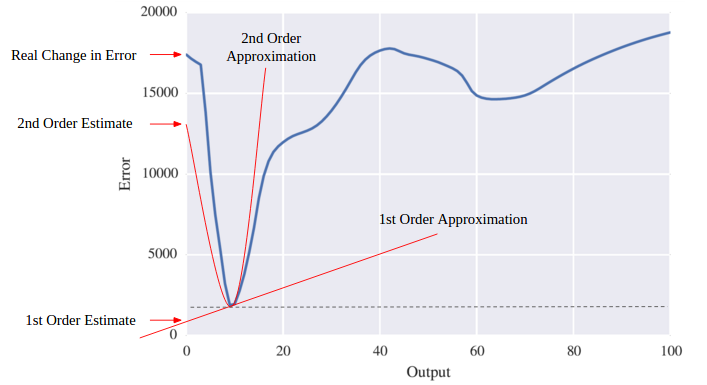
\includegraphics[width=\linewidth]{png/intuition.png}
  \caption{The intuition behind neuron pruning decision.}
  \label{fig:intuition}
\end{figure}

Figure \ref{fig:intuition} shows a random error function plotted against the output of any given neuron. Note that this figure is for illustration purposes only. The error function is minimized at a particular value of the output as can be seen in the figure. This output is fixed during training as decided by back propagation. Pruning this particular neuron would result in a change in the total error that would be equal to the increase shown in the figure. This neuron is clearly a bad candidate for removal. The straight red line in the figure represents the first-order approximation of the error using Taylor Series as described before while the parabola represents a second-order approximation. It can be clearly seen that the second-order approximation is a much better estimate of the change in error.

We would also like to point out here that it is possible in some cases that there is some thresholding required when trying to approximate the error using the 2nd order Taylor Series expansion. These cases might arise when the parabolic approximation undergoes a steep slope change. To take into account such cases, we employed mean and median thresholding, where any change above a certain threshold was assigned a mean or median value respectively.

Two pruning algorithms are proposed here. They are different in the way the neurons are ranked but both of them use $\Delta E_{k}^2$, the second-order approximation of the error function we got from the Taylor Series, as the basis for the ranking.

The first step in both the algorithms is to  decide a stopping criterion. This can vary depending on the application but some intuitive stopping criteria can be the maximum number of neurons to remove, percentage scaling needed, maximum allowable accuracy drop etc. 

\subsubsection{Algorithm I: Single Overall Ranking}
The complete algorithm is shown in Algorithm \ref{algo1}. The idea here is to generate a single ranked list based on the values of $\Delta E_{k}^2$. This involves a single pass of second-order back-propagation (without weight updates) to collect the gradients for each neuron. The neurons from the formed rank-list (with the least value of $\Delta E_{k}^2$) are then pruned according to the stopping criterion decided.

\begin{algorithm}
 \KwData{optimally trained network, training set}
 \KwResult{A pruned network}
 initialize and define stopping criterion \;
 perform forward propagation over the training set \;
  perform second-order back-propagation without updating weights and collect linear and quadratic gradients \;
  rank the remaining neurons based on $\Delta E_{k}^2$\;
 \While{stopping criterion is not met}{
  remove the last ranked neuron \;
 }
 \caption{Single Overall Ranking}
 \label{algo1}
\end{algorithm}
 
\subsubsection{Algorithm II: Iterative Re-Ranking}

In this greedy variation of the algorithm (Algorithm \ref{algo2}), after each neuron is pruned, the remaining network is made to undergo a single pass of second-order back-propagation (without weight updates) and the rank list is formed again. Hence, each removal involves a new pass through the network. This method is computationally more expensive but takes into account the dependencies the neurons might have with one another which would lead to a change in error contribution every time a dependent neuron is removed. 

\begin{algorithm}
 \KwData{optimally trained network, training set}
 \KwResult{A pruned network}
 initialize and define stopping criterion \;
 \While{stopping criterion is not met}{
  perform forward propagation over the training set \;
  perform second-order back-propagation without updating weights and collect linear and quadratic gradients \;
  rank the remaining neurons based on $\Delta E_{k}^2$  \;
  remove the worst neuron based on the ranking \;
 }
 \caption{Iterative Re-Ranking}
 \label{algo2}
\end{algorithm}

%\section{Experiments}
We propose several experiments to compare our discussed algorithm for determining which neurons to switch off with the empirically determined best ordering. First, we do brute force ordering. Using the training data, we get the sum of squared errors for the unaltered network. Then, we switch off one neuron at a time, and do one forward pass through the training data to get the change in the output error. We use this value to rank the neurons. This is the ground truth. 
\subsection{Correlation of Ranking vs. Ground Truth}
\subsection{Change in Ground Truth Error vs. Expected Improvement}
\subsection{Sequential Turn-Off}
\subsection{Iterative Re-Estimation of Next Best Neuron}
\section{Experimental Results}
\subsection{MNIST Dataset Results}
\subsubsection{Pruning A 1-Layer Network: Single-Pass Ranking}
We first present the results for a single-layer neural network in Figure \ref{fig:mnist-single-ranking-single-layer}, using a one-time computation of the overall ranking of all neurons to make our pruning decisions. After training, each neuron is assigned a permanent ranking based on three criteria: A brute force ``ground truth'' ranking, and two approximations of this ranking using first and second order Taylor estimations of the change in network output error resulting from the removal of each neuron. (We note that this algorithm is intentionally naive and is used for comparison only. Its performance should be expected to be poor.) 

\begin{figure}[!h]
\centering
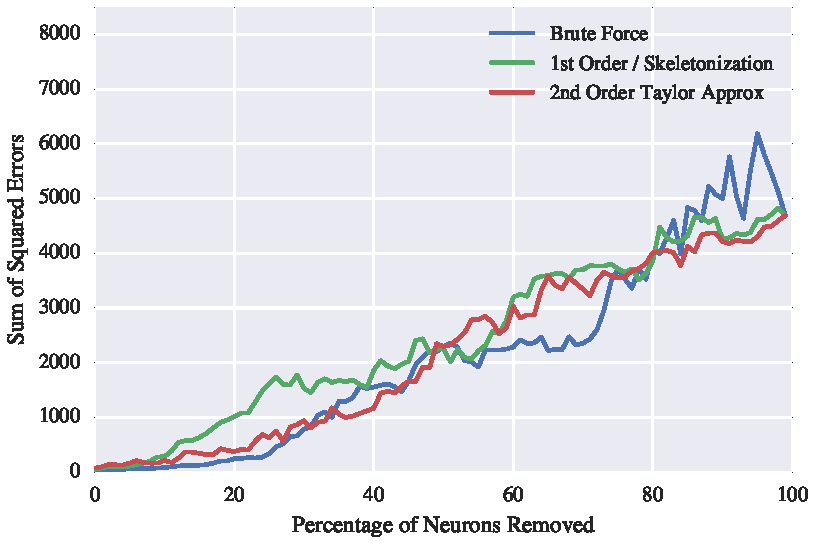
\includegraphics[width=0.49\linewidth]{png/mnist-acc99-single-pass-method.pdf}
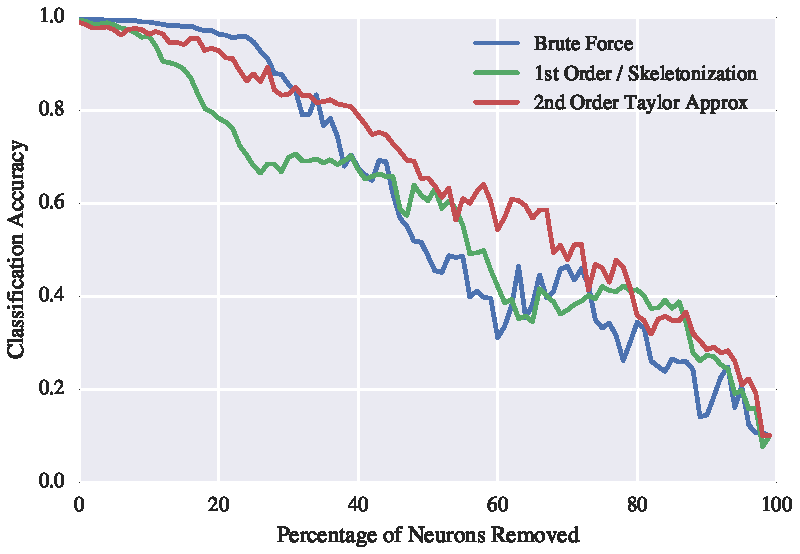
\includegraphics[width=0.49\linewidth]{png/mnist-acc99-single-pass-accuracy.pdf}
\caption{Degradation in squared error (left) and classification accuracy (right) after pruning a single-layer network trained on MNIST using a single-pass overall ranking procedure (\textbf{Network:} 1 layer, 100 neurons, 10 outputs, logistic sigmoid activation, starting test accuracy: 0.998)}
\label{fig:mnist-single-ranking-single-layer}
\end{figure}

An interesting observation here is that with only a single layer, no method for ranking the neurons in the network with a single pass emerges superior, indicating that the 1st and 2nd order methods are actually reasonable approximations of the brute force method under certain conditions. Of course, this method is still quite bad in terms of the rate of degradation of the classification accuracy and in practice we would likely follow \cite{mozer1989skeletonization}'s advice to retrain after each neuron removal in order to allow remaining neurons to adjust and compensate for network faults triggered by poor pruning decisions. The purpose of the present investigation, however, is to demonstrate how much of a trained network can be theoretically removed without altering the network's learned parameters in any way. Once again, we only present this method as a basis for comparison and we will investigate more promising methods in greater detail in later sections. 

\subsubsection{Pruning A 1-Layer Network: Re-Ranking After Each Removal}
In Figure \ref{fig:mnist-re-ranking-single-layer} we present our results using an iterative re-ranking procedure in which all remaining neurons are re-ranked after each successive neuron is switched off. We compute the same brute force rankings and Taylor series approximations of error deltas over the remaining active neurons in the network after each pruning decision. This is intended to account for the effects of canceling interactions between neurons. 

\begin{figure}[!hb]
\centering
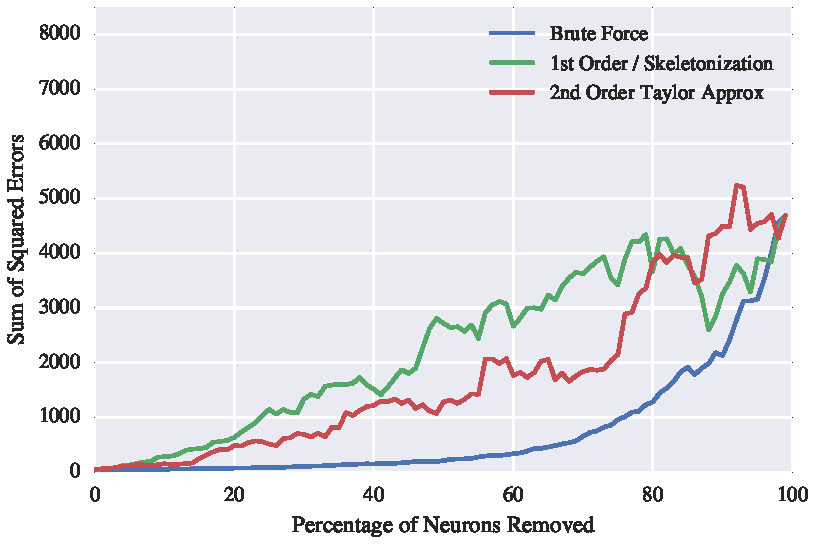
\includegraphics[width=0.49\linewidth]{png/mnist-acc99-iterative-rerank-method.pdf}
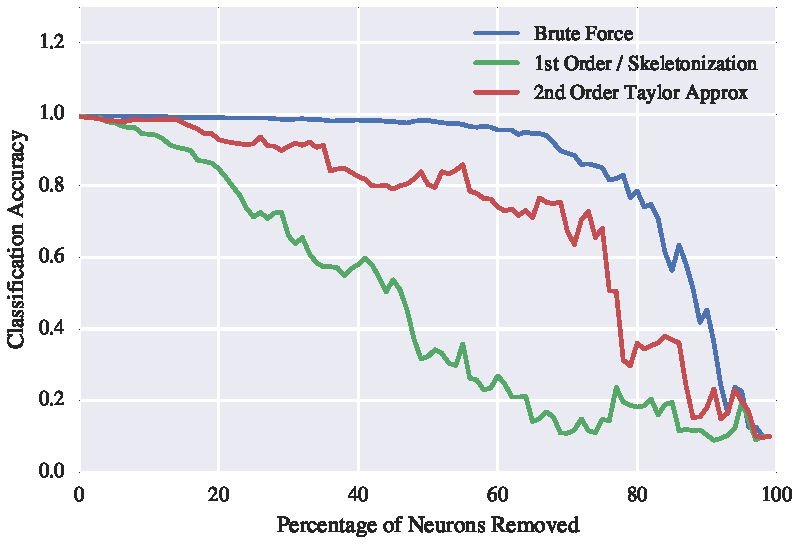
\includegraphics[width=0.49\linewidth]{png/mnist-acc99-iterative-rerank-accuracy.pdf}
\caption{Degradation in squared error (left) and classification accuracy (right) after pruning a single-layer network trained on MNIST using an iterative re-ranking procedure (\textbf{Network:} 1 layer, 100 neurons, 10 outputs, logistic sigmoid activation, starting test accuracy: 0.998)}
\label{fig:mnist-re-ranking-single-layer}
\end{figure}

tl;dr: 1 layer is grrrreat for brute force! Clearly 2nd order method is consistently better than 1st order method. 

tl;dr: Brute force method is amazing here! 1 layer makes things a lot easier, and a 2nd order method can do okay as well, but can still be improved a lot. 60% of neurons doing nothing!

\subsubsection{Visualization of Error Surface \& Pruning Decisions}
As explained in the methodology section, these graphs are a visualization the error surface of the network output with respect to the neurons chosen for removal using each algorithm, represented in intervals of 10 neurons. In each graph, the error surface of the network output is displayed in log space (left) and in real space (right) with respect to each candidate neuron chosen for removal. We create these plots during the pruning exercise by picking a neuron to switch off, and then multiplying its output by a scalar gain value $\alpha$ which is adjusted from 0.0 to 10.0 with a step size of 0.001. When the value of $\alpha$ is 1.0, this represents the unperturbed neuron output learned during training. Between 0.0 and 1.0, we are graphing the literal effect of turning the neuron off ($\alpha = 0$), and when $\alpha > 1.0$ we are simulating a boosting of the neuron's influence in the network, i.e. inflating the value of its outgoing weight parameters. 

We graph the effect of boosting the neuron's output to demonstrate that for certain neurons in the network, even doubling, tripling, or quadrupling the scalar output of the neuron has no effect on the overall error of the network, indicating the remarkable degree to which the network has learned to ignore the value of certain parameters. In other cases, we can get a sense of the sensitivity of the network's output to the value of a given neuron when the curve rises steeply after the red 1.0 line. This indicates that the learned value of the parameters emanating from a given neuron are relatively important, and this is why we should ideally see sharper upticks in the curves for the later-removed neurons in the network, that is, when the neurons crucial to the learning representation start to be picked off. 

Remember that lower is better in terms of the height of the curve and minimal horizontal change between the vertical red line at 1.0 (neuron \textit{on}, $\alpha = 1.0$) and 0.0 (neuron \textit{off}, $\alpha = 0.0$) is indicative of a good candidate neuron to prune, i.e. there will be minimal effect on the network output when the neuron is removed. The network architecture in this case consisted of 1 layer, 100 neurons, 10 outputs, logistic sigmoid activations, and a starting test accuracy of 0.998.

\textbf{Brute Force Method}
\begin{figure}[!hb]
\centering
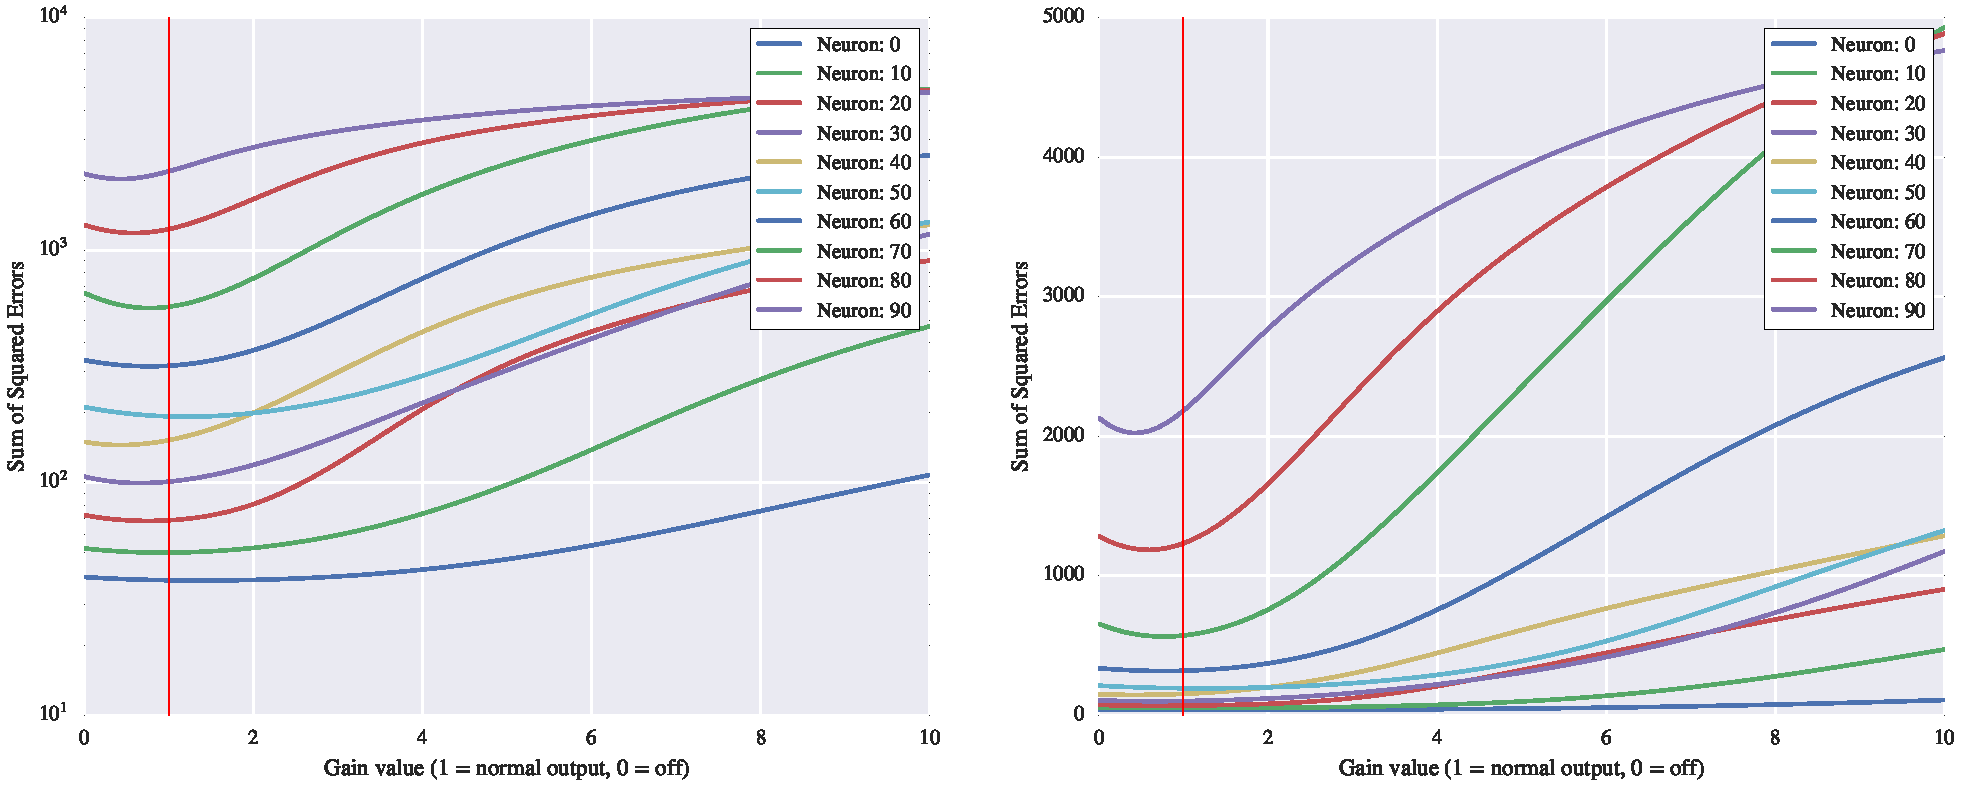
\includegraphics[width=\linewidth]{png/mnist-acc99-gt-gain.pdf}
\caption{Error surface of the network output in log space (left) and in real space (right) with respect to each candidate neuron chosen for removal; (\textbf{Network:} 1 layer, 100 neurons, 10 outputs, logistic sigmoid activation, starting test accuracy: 0.998)}
\label{fig:mnist-gt-single-layer}
\end{figure}
tl;dr: Notice how low to the floor and flat most of these curves are. It's only until the 90th removed neuron that we see a higher cure with a more convex shape (clearly a more influential piece of the network)

\textbf{1st Order Method}
\begin{figure}[!hb]
\centering
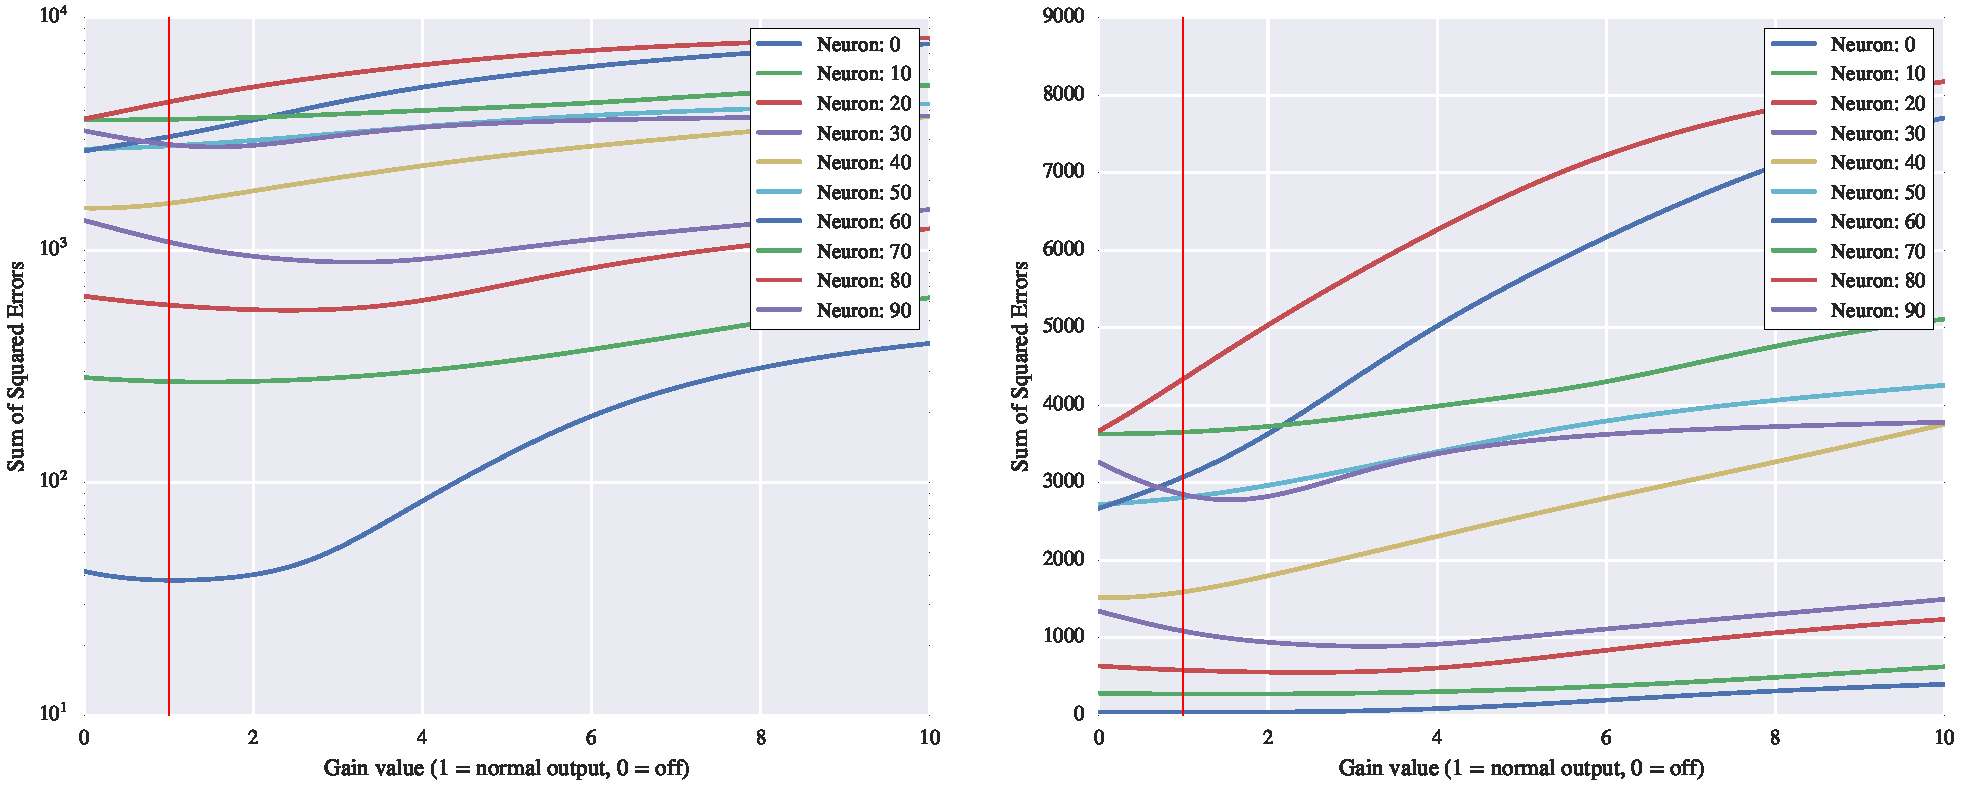
\includegraphics[width=\linewidth]{png/mnist-acc99-g1-gain.pdf}
\caption{Error surface of the network output in log space (left) and in real space (right) with respect to each candidate neuron chosen for removal; (\textbf{Network:} 1 layer, 100 neurons, 10 outputs, logistic sigmoid activation, starting test accuracy: 0.998)}
\label{fig:mnist-gt-single-layer}
\end{figure}
tl;dr: Most choices seem to have flat or negatively sloped curves, indicating that the first order approx seems to be pretty good, but examining the brute force choices shows they could be better. 

\textbf{2nd Order Method}
\begin{figure}[!hb]
\centering
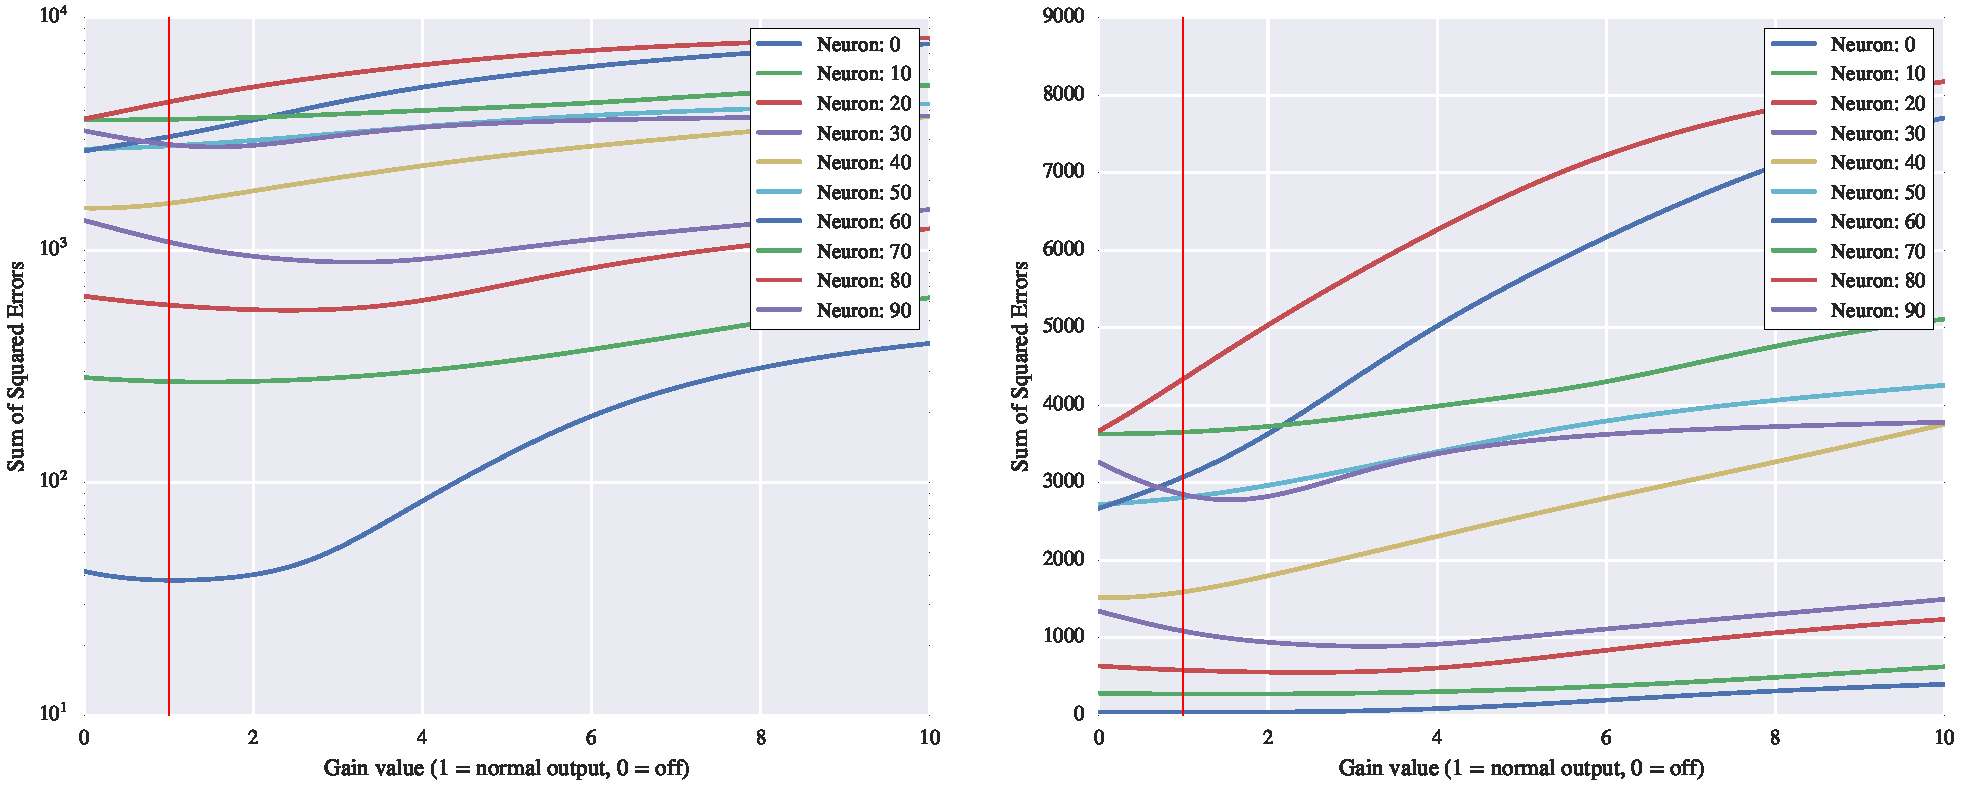
\includegraphics[width=\linewidth]{png/mnist-acc99-g1-gain.pdf}
\caption{Error surface of the network output in log space (left) and in real space (right) with respect to each candidate neuron chosen for removal; (\textbf{Network:} 1 layer, 100 neurons, 10 outputs, logistic sigmoid activation, starting test accuracy: 0.998)}
\label{fig:mnist-gt-single-layer}
\end{figure}
tl;dr: Looks much more similar to the Brute Force method choices, though clearly not as good (they're more spread out). Notice the difference in convexity between the 2nd and 1st order method choices. It's clear that the first order method is fitting a line and the 2nd order method is fitting a parabola in their approximation. 

\subsubsection{Pruning A 2-Layer Network: Single-Pass Ranking}
Figure \ref{fig:mnist-single-ranking-double-layer} shows the result of using a one-time computation of the overall ranking of all neurons to make pruning decisions for a two-layer network. The ranking procedure is identical to the one used to generate Figure \ref{fig:mnist-single-ranking-single-layer}. (We again note that this algorithm is intentionally naive and is used for comparison only. Its performance should be expected to be poor.) 

\begin{figure}[!hb]
\centering
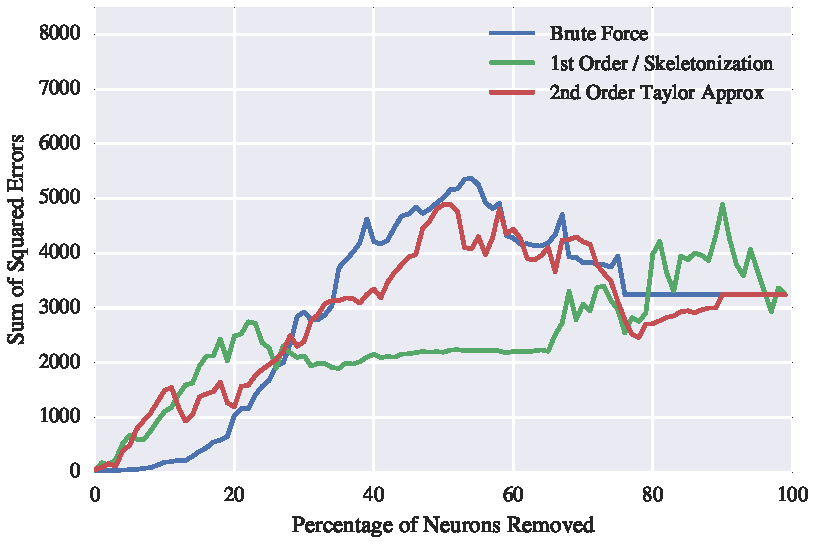
\includegraphics[width=0.49\linewidth]{png/mnist-deep-single-pass-method.pdf}
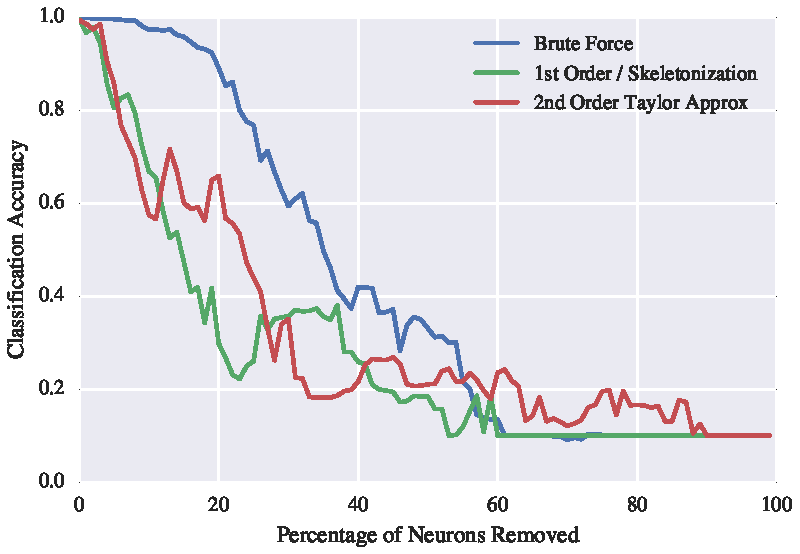
\includegraphics[width=0.49\linewidth]{png/mnist-deep-single-pass-accuracy.pdf}
\caption{Degradation in squared error (left) and classification accuracy (right) after pruning a 2-layer network trained on MNIST using a single-pass overall ranking procedure (\textbf{Network:} 2 layers, 50 neurons/layer, 10 outputs, logistic sigmoid activation, starting test accuracy: 1.000)}
\label{fig:mnist-single-ranking-double-layer}
\end{figure}

tl;dr: Unsurprisingly, a 2-layer network is harder to prune because a single overall ranking will never capture the interdependencies between neurons in different layers. It makes sense that this is much worse than the performance on the 1-layer network, even if this method is already known to be bad, and we'd likely never use it in practice. 


\subsubsection{Pruning A 2-Layer Network: Re-Ranking After Each Removal}
Figure \ref{fig:mnist-re-ranking-double-layer} shows the results results using an iterative re-ranking procedure on a two-layer network. We compute the same brute force rankings and Taylor series approximations of error deltas over the remaining active neurons in the network after each pruning decision used to generate Figure \ref{fig:mnist-re-ranking-single-layer}. Again, this is intended to account for the effects of canceling interactions between neurons. 

\begin{figure}[!hb]
\centering
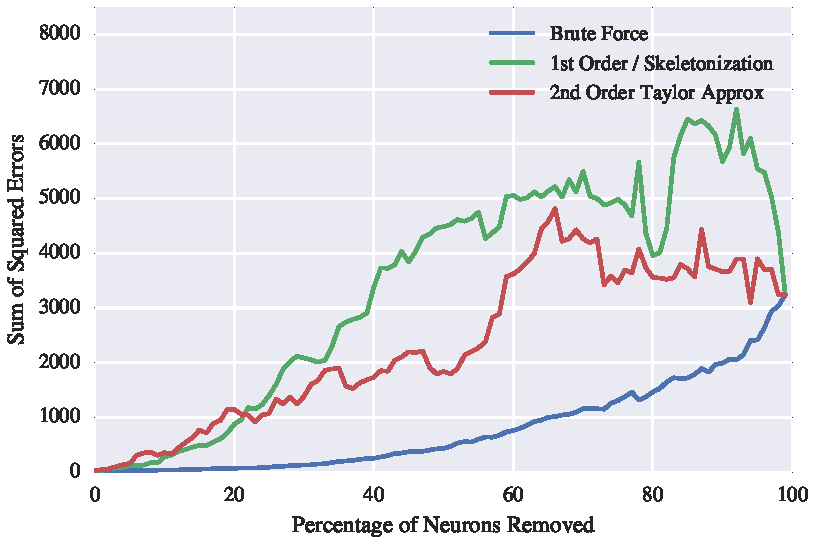
\includegraphics[width=0.49\linewidth]{png/mnist-deep-iterative-rerank-method.pdf}
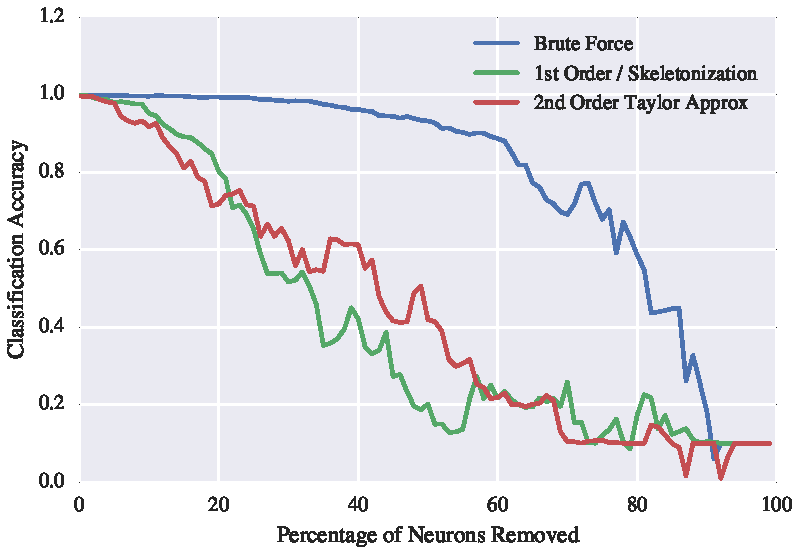
\includegraphics[width=0.49\linewidth]{png/mnist-deep-iterative-rerank-accuracy.pdf}
\caption{Degradation in squared error (left) and classification accuracy (right) after pruning a 2-layer network trained on MNIST using an iterative re-ranking procedure (\textbf{Network:} 2 layers, 50 neurons/layer, 10 outputs, logistic sigmoid activation, starting test accuracy: 1.000)}
\label{fig:mnist-re-ranking-double-layer}
\end{figure}

tl;dr: clearly a higher set of curves, indicating that it becomes harder to remove neurons 1-by-1 with a deeper network (which makes sense because the neurons have more interdependencies in a deeper network), but we see an overall better performance with 2nd order method vs. 1st order, except for the first 20% of the neurons (but this doesn't seem to make much difference for classification accuracy.) 

tl;dr: Shows the clear potential of an ideal pruning technique, and how inconsistent 1st and 2nd order methods can be

\subsubsection{Visualization of Error Surface \& Pruning Decisions}
These graphs are a visualization the error surface of the network output with respect to the neurons chosen for removal using each algorithm, represented in intervals of 10 neurons. 

\textbf{Brute Force Method}
\begin{figure}[!hb]
\centering
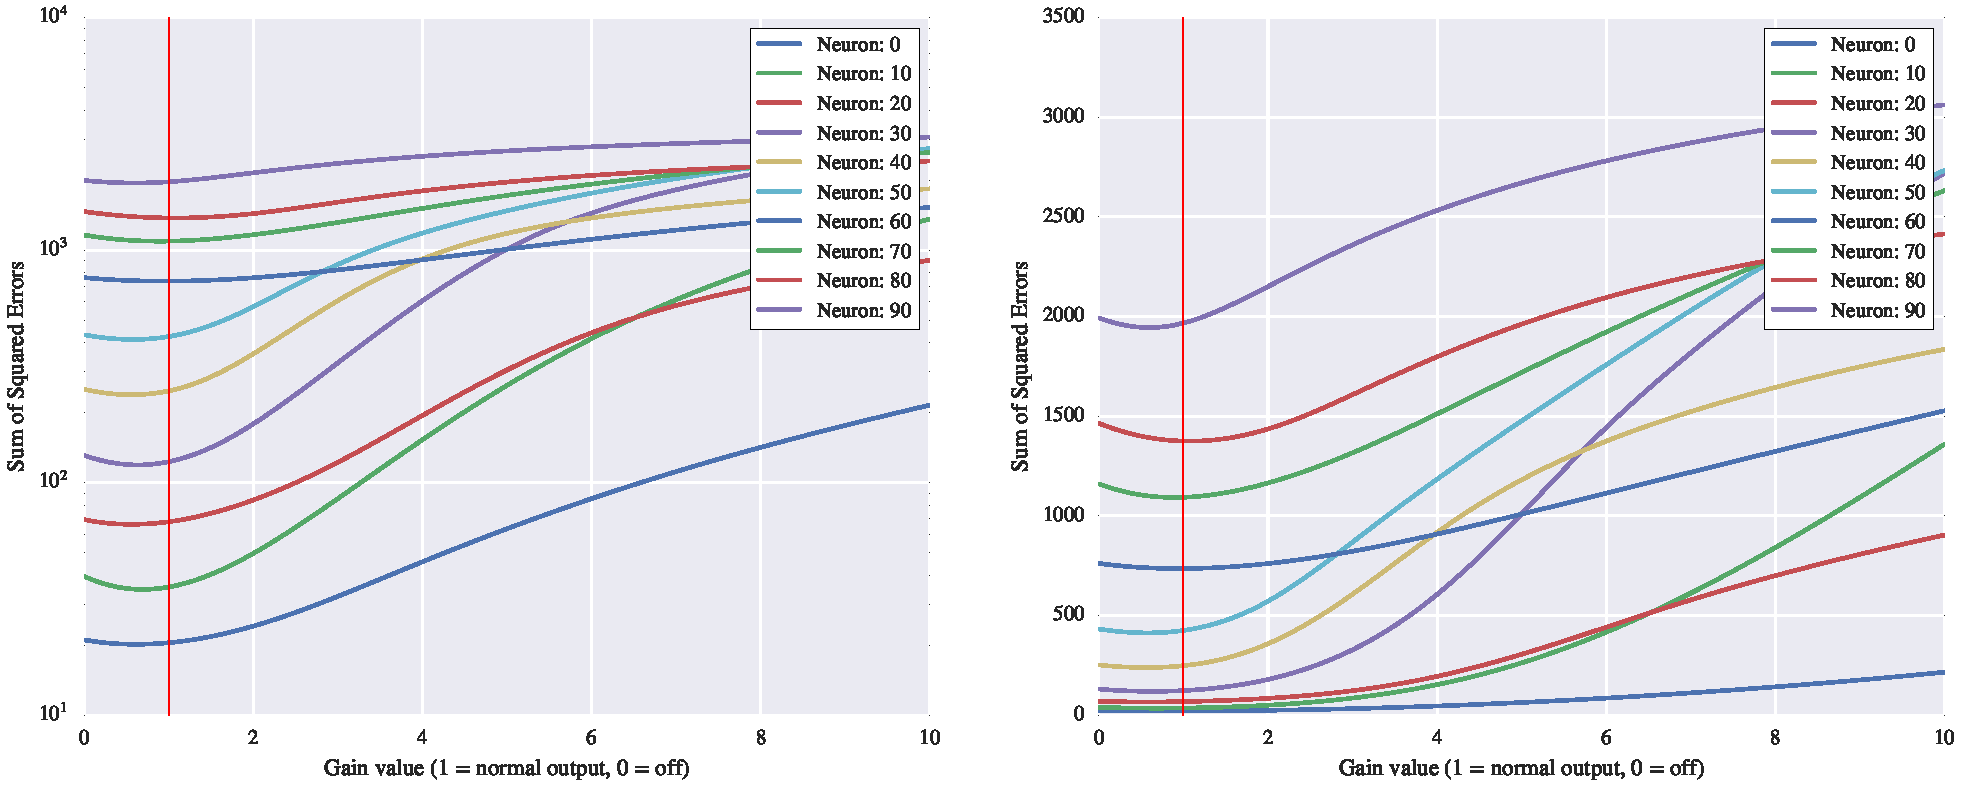
\includegraphics[width=\linewidth]{png/mnist-deep-gt-gain.pdf}
\caption{Error surface of the network output in log space (left) and in real space (right) with respect to each candidate neuron chosen for removal; (\textbf{Network:} 2 layers, 50 neurons/layer, 10 outputs, logistic sigmoid activation, starting test accuracy: 1.000)}
\label{fig:mnist-gt-double-layer}
\end{figure}
tl;dr: It's clear why these neurons were chosen, their graphs clearly show little change when neuron is removed, are mostly near the floor, and show convex behavior of error surface, which argues for the rationalization of using 2nd order methods to estimate difference in error when they are turned off

\textbf{1st Order Method}
\begin{figure}[!hb]
\centering
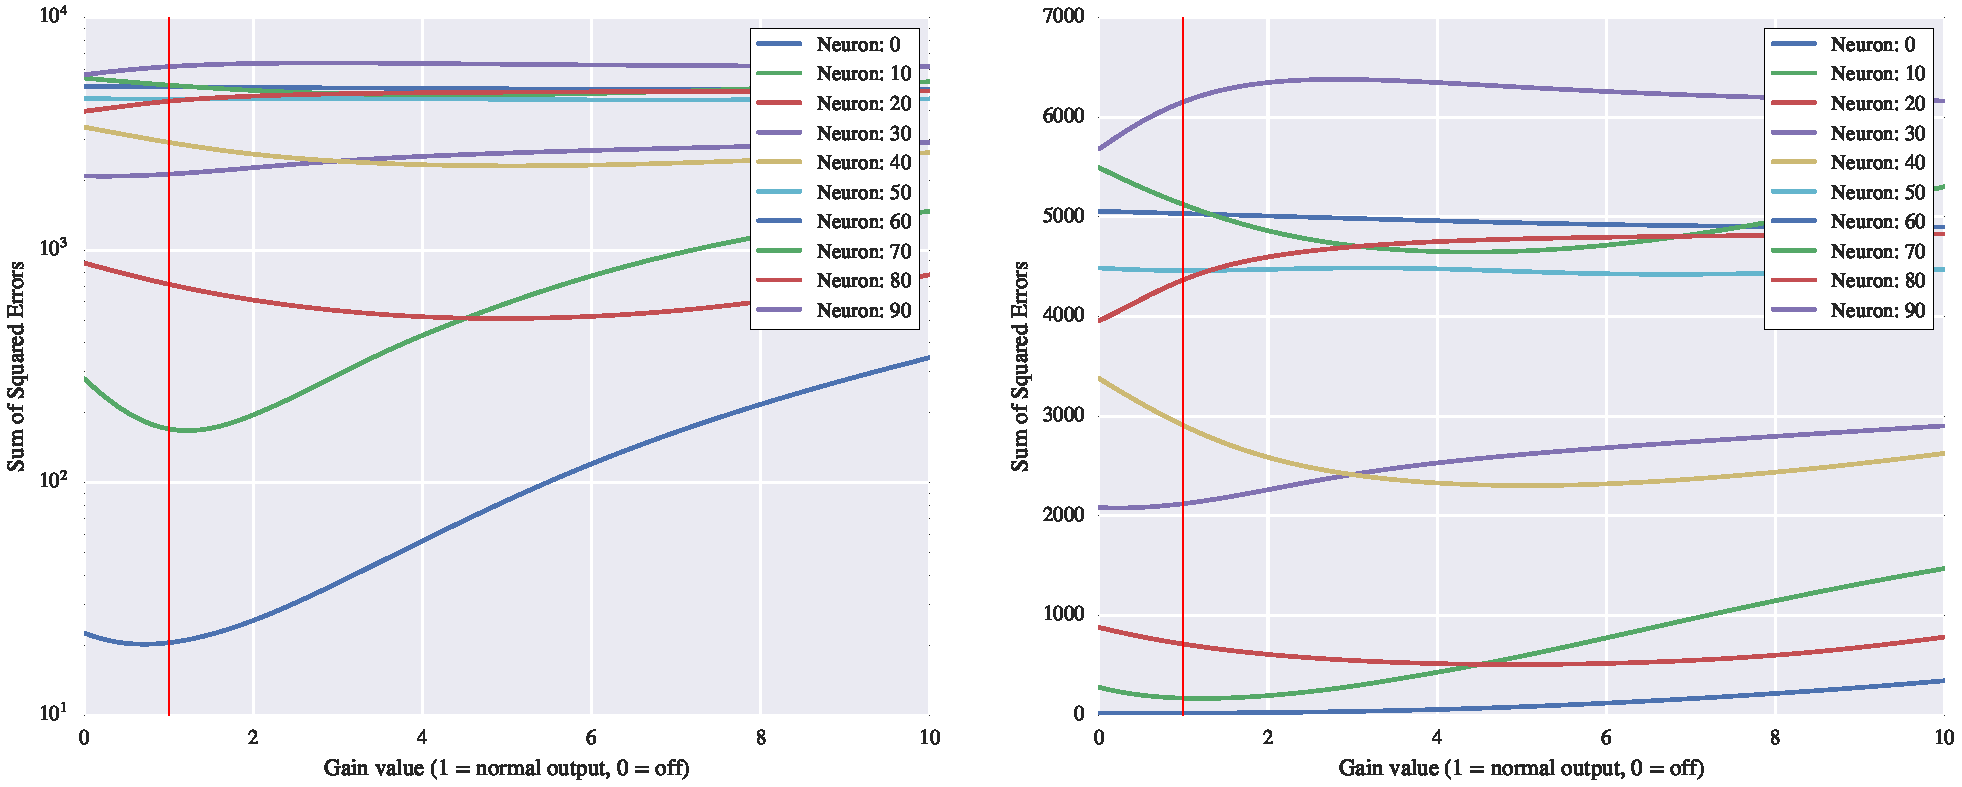
\includegraphics[width=\linewidth]{png/mnist-deep-g1-gain.pdf}
\caption{Error surface of the network output in log space (left) and in real space (right) with respect to each candidate neuron chosen for removal; (\textbf{Network:} 2 layers, 50 neurons/layer, 10 outputs, logistic sigmoid activation, starting test accuracy: 1.000)}
\label{fig:mnist-g1-double-layer}
\end{figure}
 tl;dr: Drawing flat line at the point of each neurons intersection with the red vertical line (no change in gain) shows that the 1st derivative method is actually accurate for estimation of change in error in these cases, but still ultimately leads to poor decisions. 

\textbf{2nd Order Method}
\begin{figure}[!hb]
\centering
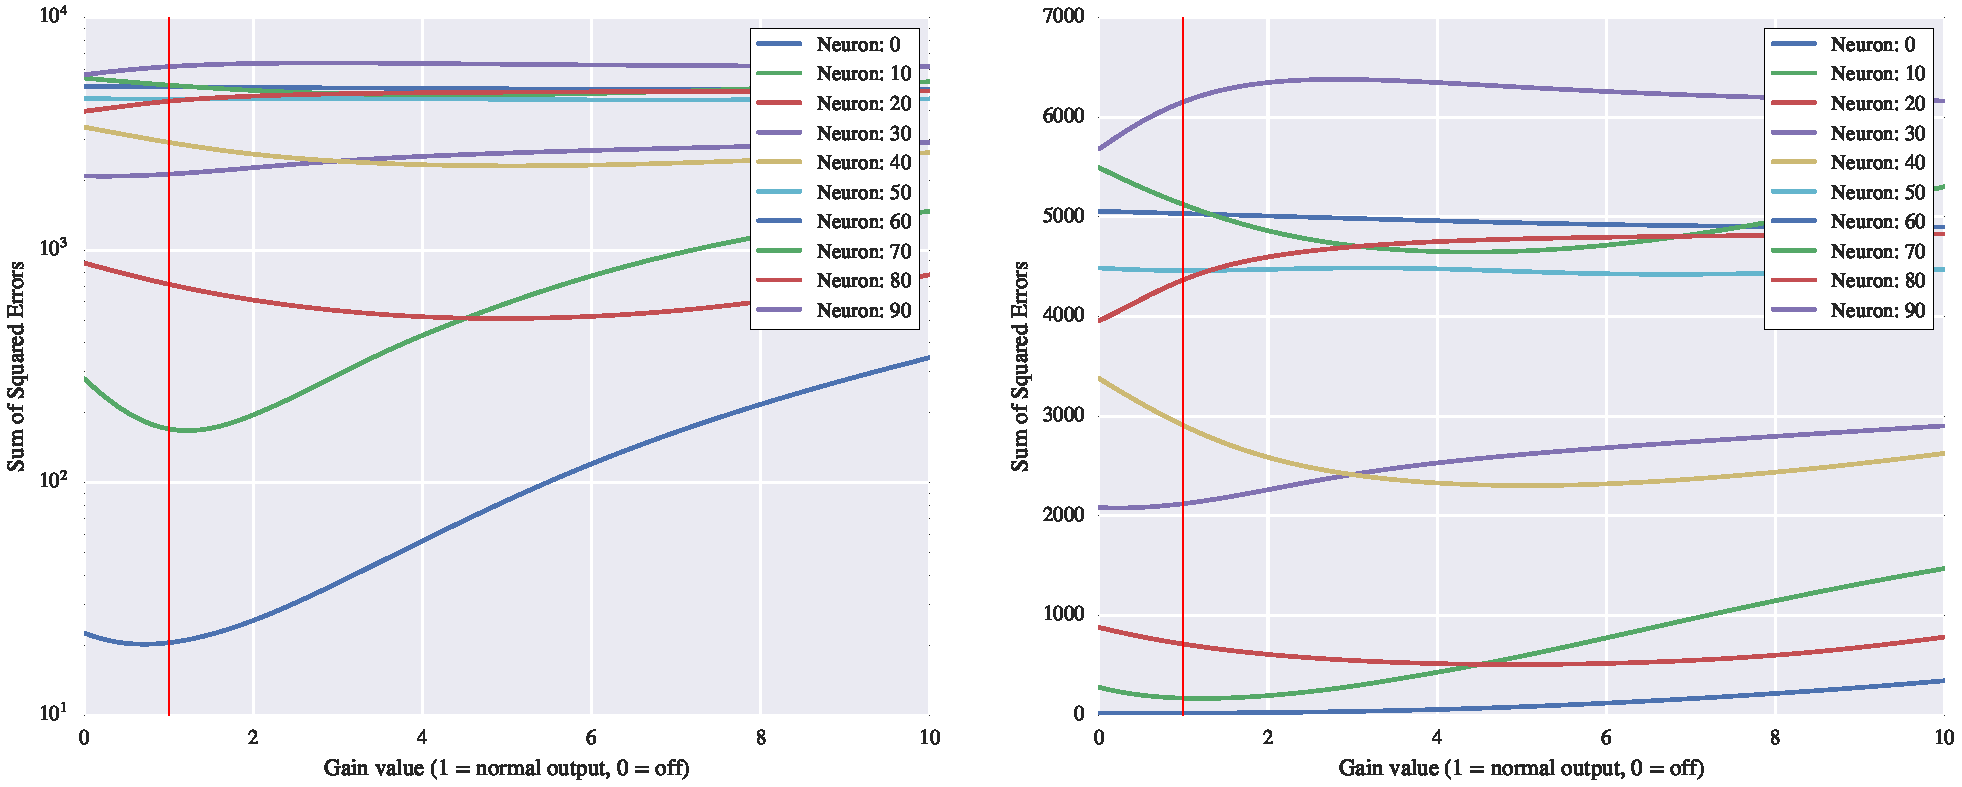
\includegraphics[width=\linewidth]{png/mnist-deep-g1-gain.pdf}
\caption{Error surface of the network output in log space (left) and in real space (right) with respect to each candidate neuron chosen for removal; (\textbf{Network:} 2 layers, 50 neurons/layer, 10 outputs, logistic sigmoid activation, starting test accuracy: 1.000)}
\label{fig:mnist-g2-double-layer}
\end{figure}
tl;dr: Clearly these are not overtly poor candidates for removal (error doesn't change much between 1.0 \& zero-crossing left-hand-side), but could be better (see brute force)

\section{Discussion of Results}

 * first or second layer?
 * cascade correlation in reverse?
 * retraining?
 * investigation of the true independence of the elements

\section{Conclusions \& Future Work}

\subsection{Conclusions}
2nd-Order Method Consistently better than 1st-Order, but still pretty bad
Both Methods fail miserably beyond the 1st layer in terms of classification accuracy
For the 2-layer networks the 1st/2nd order methods do not appear to have any apparent preference for the 1st or 2nd layer in pruning decisions. 
Brute force method pulls primarily from the outer layer at the beginning -- clearly the 1st and 2nd order methods will suffer from their difference in this regard
Performance is worse if initial network is not trained to near-perfect accuracy, but pruning in this case typically improves MSE (not accuracy) for the first 5-10% of neurons removed
Brute force method is surprisingly good and indicates the degree to which extra parameters are a waste
Sum of squared errors is a decent proxy for classification accuracy, but classification accuracy is a clearer signal of performance in such problems
If Brute Force method were made comutationally viable, could be used to prune 40-80% of neurons in almost all cases with NO re-training
This empirically shows that the learning representation is not evenly distributed over neurons, indicating NO advantage to larger networks if unnecessary
Confirms Mozer \& Smolensky's conclusion in 1989: Learning representation NOT distributed!
Neurons clearly group together to cancel out each other's effects (see spikes in classification accuracy drop-off graphs), which means neural networks use a few neurons to learn the function approximation, and the rest cooperate to cancel out each other's effects!

* second derivative method works better
* still not very good
* retraining is a good idea
* speedup of brute force method
* which layer gets pruned first

\subsection{Future Work}
Future experiments (NOT for this paper):
Try with deeper networks (3/4/5 layers) to see if the performance degrades as we should expect
Speed up brute force method through parallelization?
How do results improve when we re-train after pruning 1-n neurons in a row? (expectation: smooooooooth curve for brute force method)
Examine whether Cascade Correlation arrives at the same minimal number of neurons
Use cross entropy to make pruning decision for classification problems
Try a regression task on a real-world dataset, e.g. housing prices, stock market, etc. 

\section*{Acknowledgments}
We would like to thank Lukas Drude for the assistance with calculations on collecting quadratic error gradients through the 2nd order version of back-propagation. We would also like to thank Rita Singh, Abelino Jiminez, Thomas Schaaf and Don Wolfe for helpful discussions.

%\pagebreak
\section{Appendix A: Second Derivative Back-Propagation}
Name and network definitions:\\
\begin{align}
E &= \frac{1}{2}\sum\limits_i (\Out i 0 - \Target i)^2 &
\Out i m &= \sigma(\Input i m) &
\Input i m &= \sum\limits_j {\Weight j i m}{ \Out j {m + 1}} &
\Con j i m = \Weight j i m \Out j {m+1}
\end{align}
Superscripts represent the index of the layer of the network in question, with 0 representing the output layer. $E$ is the squared-error network cost function. $\Out i m$ is the $i$th output in layer $m$ generated by the activation function $\sigma$, which in this paper is is the standard logistic sigmoid. $\Input i m$ is the weighted sum of inputs to the $i$th neuron in the $m$th layer, and $\Con j i m$ is the contribution of the $j$th neuron in the $m+1$ layer to the input of the $i$th neuron in the $m$th layer. 
\subsection{First and Second Derivatives} 
The first and second derivatives of the cost function with respect to the outputs:
\begin{align}
\pdv{E}{\Out i 0} &= \Out i 0 - \Target i \label{cost_func_derivative}
\end{align}
\begin{align}
\pdv[2]{E}{{\Out i 0}} &= 1\label{cost_func_2nd_derivative}
\end{align}
The first and second derivatives of the sigmoid function in forms depending only on the output:
\begin{align}
\sigma^{\prime}(x) &= \sigma(x)\left(1 - \sigma(x)\right)\label{sigmoid_derivative} 
\\
\sigma^{\prime\prime}(x) &= \sigma^{\prime}(x)\left(1 - 2\sigma(x)\right) \label{sigmoid_2nd_derivative}
\end{align}
The second derivative of the sigmoid is easily derived from the first derivative:
\begin{align}
\sigma^{\prime}(x) &= \sigma(x)\left(1 - \sigma(x)\right)
\\
\sigma^{\prime\prime}(x) &= \dv{}{x}
\underbrace{\sigma(x)}_{f(x)}
\underbrace{\left(1 - \sigma(x)\right)}_{g(x)}
\\
\sigma^{\prime\prime}(x) &= f^{\prime}(x)g(x) + f(x)g^{\prime}(x)
\\
\sigma^{\prime\prime}(x) &= \sigma^{\prime}(x)(1-\sigma(x)) - \sigma(x)\sigma^{\prime}(x)
\\
\sigma^{\prime\prime}(x) &= \sigma^{\prime}(x) - 2\sigma(x)\sigma^{\prime}(x)
\\
\sigma^{\prime\prime}(x) &= \sigma^{\prime}(x)(1 - 2\sigma(x))
\end{align}

And for future convenience: 
\begin{align}
\dv{\Out i m}{\Input i m} &= 
\dv{}{\Input i m}\left({\Out i m} = \sigma(\Input i m)\right) 
\\
&= \left(\Out i m\right)\left(1 - \Out i m\right)
\\
&= \sigma^{\prime}\left(\Input i m\right)
\\
\dv[2]{{\Out i m}}{{\Input i m}} &=
\dv{}{{\Input i m}}\left(\dv{\Out i m}{\Input i m} = \left(\Out i m\right)\left(1 - \Out i m\right)\right)
\\
&= \left(\Out i m\left(1 - \Out i m\right)\right)\left(1 - 2\Out i m\right)
\\
&= \sigma^{\prime\prime}\left(\Input i m\right)
\end{align}

Derivative of the error with respect to the $i$th neuron's input $\Input i 0$ in the output layer:
\begin{align}
\pdv{E}{\Input i 0} &= \pdv{E}{\Out i 0} \pdv{\Out i 0}{\Input i 0} 
\\
&= \underbrace{\left(\Out i 0 - \Target i\right)}_{\text{from} \ (\ref{cost_func_derivative})} \underbrace{\sigma\left(\Input i 0\right)\left(1 - \sigma\left(\Input i 0\right)\right)}
_{\text{from} \ (\ref{sigmoid_derivative})}
\\
&= \left(\Out i 0 - \Target i\right)\left(\Out i 0 \left(1 - \Out i 0\right)\right)
\\
&= \left(\Out i 0 - \Target i\right)\sigma^{\prime}\left(\Input i 0\right)\label{dedx}
\end{align}

Second derivative of the error with respect to the $i$th neuron's input $\Input i 0$ in the output layer:
\begin{align}
\pdv[2]{E}{{\Input i 0}} &= \pdv{}{\Input i 0}
\left(\pdv{E}{\Out i 0}\pdv{\Out i 0}{\Input i 0}\right) 
\\
&= \pdv{E}{\Input i 0}{\Out i 0}
\pdv{\Out i 0}{\Input i 0} + \pdv{E}{\Out i 0}\pdv[2]{\Out i 0}{{\Input i 0}}
\\
&= \pdv{E}{\Input i 0}{\Out i 0}
\underbrace{\left(\Out i 0 \left(1 - \Out i 0\right)\right)}_{{\text{from} \ (\ref{sigmoid_derivative})}} + \underbrace{\left(\Out i 0 - \Target i\right)}_{\text{from} \ (\ref{cost_func_derivative})}\underbrace{\left(\Out i 0 \left(1 - \Out i 0\right)\right)\left(1 - 2\Out i 0\right) }_{\text{from}\ (\ref{sigmoid_2nd_derivative})}
\\
\left(\pdv{E}{\Input i 0}{\Out i 0}\right)
&= \pdv{}{\Input i 0}\pdv{E}{\Out i 0} = \pdv{}{\Input i 0}\underbrace{\left(\Out i 0 - \Target i\right)}_{\text{from} \ (\ref{cost_func_derivative})} = \pdv{\Out i 0}{\Input i 0} = \underbrace{\left(\Out i 0 \left(1 - \Out i 0\right)\right)}_{{\text{from} \ (\ref{sigmoid_derivative})}} 
\\
\pdv[2]{E}{{\Input i 0}}&= \left(\Out i 0 \left(1 - \Out i 0\right)\right)^2 + \left(\Out i 0 - \Target i\right)\left(\Out i 0 \left(1 - \Out i 0\right)\right)\left(1 - 2\Out i 0\right) 
\\
&= \left(\sigma^{\prime}\left(\Input i 0\right)\right)^2 + \left(\Out i 0 - \Target i\right)\sigma^{\prime\prime}\left(\Input i 0\right)\label{d2edx2}
\end{align}

First derivative of the error with respect to a single input contribution $\Con j i 0$ from neuron $j$ to neuron $i$ with weight $\Weight j i 0$ in the output layer:
\begin{align}
\pdv{E}{\Con j i 0} &= 
\pdv{E}{\Out i 0}
\pdv{\Out i 0}{\Input i 0}
\pdv{\Input i 0}{\Con j i 0}
\\
&= \underbrace{\left(\Out i 0 - \Target i \right)}_{\text{from} \ (\ref{cost_func_derivative})} \underbrace{\left(\Out i 0 \left(1 - \Out i 0\right) \right)}_{\text{from} \ (\ref{sigmoid_derivative})} \pdv{\Input i 0}{\Con j i 0} 
\\
\left( \pdv{\Input i m}{\Con j i m}\right) &= \pdv{}{\Con j i m}\left(\Input i m = \sum_j\Weight j i m\Out j {m+1} \right) = \pdv{}{\Con j i m} \left(\Con j i m + k \right) = 1\label{dxdc} 
\\
\pdv{E}{\Con j i 0}&= \left(\Out i 0 - \Target i \right) \left(\Out i 0 \left(1 - \Out i 0\right) \right)
\\
&= \underbrace{\left(\Out i 0 - \Target i \right) \sigma^{\prime}\left(\Input i 0\right)\label{dedc}}
_{\text{from} \ (\ref{dedx})} 
\\
\pdv{E}{\Con j i 0} &= \pdv{E}{\Input i 0}
\end{align}

Second derivative of the error with respect to a single input contribution $\Con j i 0$:
\begin{align}
\pdv[2]{E}{{\Con j i 0}} &=
\pdv{}{\Con j i 0} 
\left(\pdv{E}{\Con j i 0} = 
\underbrace{\left(\Out i 0 - \Target i \right) \sigma^{\prime}\left(\Input i 0\right)}
_{\text{from} \ (\ref{dedc})}
\right)
\\
&=\pdv{}{\Con j i 0}\left(\sigma\left(\Input i 0\right) - \Target i \right) \sigma^{\prime}\left(\Input i 0\right)
\\
&=\pdv{}{\Con j i 0}\left(\sigma\left(\sum\limits_j {\Weight j i m}{ \Out j {m + 1}}\right) - \Target i \right) \sigma^{\prime}\left(\sum\limits_j {\Weight j i m}{ \Out j {m + 1}}\right)
\\
&=\pdv{}{\Con j i 0}\left(\sigma\left(\sum\limits_j {\Con j i 0}\right) - \Target i \right) \sigma^{\prime}\left(\sum\limits_j {\Con j i 0}\right)
\\
&=\pdv{}{\Con j i 0}
\underbrace{\left(\sigma\left({\Con j i 0} + k\right) - \Target i \right)}
_{f\left(\Con j i 0\right)}
\underbrace{\sigma^{\prime}\left({\Con j i 0} + k\right)}
_{g\left(\Con j i 0\right)}
\end{align}

We now make use of the abbreviations $f$ and $g$:
\begin{align}
&=f^{\prime}\left(\Con j i 0\right)g\left(\Con j i 0\right) + f\left(\Con j i 0\right)g^{\prime}\left(\Con j i 0\right)
\\
&=\sigma^{\prime}\left({\Con j i 0} + k\right)\sigma^{\prime}\left({\Con j i 0} + k\right) + 
\left(\sigma\left({\Con j i 0} + k\right) - \Target i \right)\sigma^{\prime\prime}\left({\Con j i 0} + k\right)
\\
&=\sigma^{\prime}\left({\Con j i 0} + k\right)^2 + 
\left(\Out i 0 - \Target i \right)\sigma^{\prime\prime}\left({\Con j i 0} + k\right)
\\
&\left(\Con j i 0 + k = \sum_j{\Con j i 0} = \sum\limits_j {\Weight j i m}{ \Out j {m + 1}} = \Input i 0 \right)
\\
\pdv[2]{E}{{\Con j i 0}}&=
\underbrace{\left(\sigma^{\prime}\left(\Input i 0\right)\right)^2 + 
\left(\Out i 0 - \Target i \right)\sigma^{\prime\prime}\left(\Input i 0\right)}
_{\text{from} \ (\ref{d2edx2})}
\\
\pdv[2]{E}{{\Con j i 0}} &= \pdv[2]{E}{{\Input i 0}}
\end{align}


\subsubsection{Summary Of Output Layer Derivatives}
\begin{align}
&\pdv{E}{\Out i 0} = \Out i 0 - \Target i 
&
\pdv[2]{E}{{\Out i 0}} = 1
\end{align}
\begin{align}
&\pdv{E}{\Input i 0} = \left(\Out i 0 - \Target i\right)\sigma^{\prime}\left(\Input i 0\right)
& 
\pdv[2]{E}{{\Input i 0}} = \left(\sigma^{\prime}\left(\Input i 0\right)\right)^2 + \left(\Out i 0 - \Target i\right)\sigma^{\prime\prime}\left(\Input i 0\right)
\end{align}
\begin{align}
&\pdv{E}{{\Con j i 0}} = \pdv{E}{{\Input i 0}}
&
\pdv[2]{E}{{\Con j i 0}} = \pdv[2]{E}{{\Input i 0}}
\end{align}


\subsubsection{Hidden Layer Derivatives}
The first derivative of the error with respect to a neuron with output $\Out j 1$ in the first hidden layer, summing over all partial derivative contributions from the output layer:
\begin{align}
\pdv{E}{\Out j 1} &= 
\sum_i
\pdv{E}{\Out i 0}
\pdv{\Out i 0}{\Input i 0}
\pdv{\Input i 0}{\Con j i 0}
\pdv{\Con j i 0}{\Out j 1}
= 
\sum_i
\underbrace{\left(\Out i 0 - \Target i\right)\sigma^{\prime}\left(\Input i 0\right)}
_{\text{from} \ (\ref{dedx})}
\Weight j i 0
\\
&\pdv{{\Con j i m}}{{\Out j {m+1}}} = \pdv{}{{\Out j {m+1}}}\left(\Con j i m = \Weight j i m\Out j {m+1}\right) = \Weight j i m\label{dcdo}
\\
\pdv{E}{\Out j 1} &= \sum_i\pdv{E}{\Input i 0}\Weight j i 0
\end{align}
Note that this equation does not depend on the specific form of $\pdv{E}{\Input i 0}$, whether it involves a sigmoid or any other activation function. We can therefore replace the specific indexes with general ones, and use this equation in the future.
\begin{align}
\pdv{E}{\Out j {m+1}} &= \sum_i\pdv{E}{\Input i m}\Weight j i m\label{dedo_general}
\end{align}
The second derivative of the error with respect to a neuron with output $\Out j 1$ in the first hidden layer:
\begin{align}
\pdv[2]{E}{{\Out j 1}} &= 
\pdv{}{\Out j 1}
\pdv{E}{\Out j 1}
\\
&= \pdv{}{\Out j 1}
\sum_i\pdv{E}{\Input i 0}\Weight j i 0
\\
&= \pdv{}{\Out j 1}
\sum_i
\left(\Out i 0 - \Target i\right)\sigma^{\prime}\left(\Input i 0\right)\Weight j i 0
\end{align}

If we now make use of the fact, that 
${\Out i 0} = \sigma\left({\Input i 0}\right) = \sigma\left(\sum_j\left({\Weight j i 0}{\Out j 1}\right)\right)$, we can evaluate the expression further.

\begin{align}
\pdv[2]{E}{{\Out j 1}}
&= \pdv{}{\Out j 1}
\sum_i
\underbrace{\left(\sigma\left(\sum_j{\Weight j i 0}{\Out j 1}\right) - \Target i\right)}
_{f\left(\Out j 1\right)}
\underbrace{\sigma^{\prime}\left(\sum_j{\Weight j i 0}{\Out j 1}\right)\Weight j i 0}
_{g\left(\Out j 1\right)}
\\
&=\sum_i\left(f^{\prime}\left(\Out j 1\right)g\left(\Out j 1\right) + f\left(\Out j 1\right)g^{\prime}\left(\Out j 1\right)\right)
\\
&=\sum_i
\sigma^{\prime}\left(\sum_j{\Weight j i 0}{\Out j 1}\right)\Weight j i 0 \
\sigma^{\prime}\left(\sum_j{\Weight j i 0}{\Out j 1}\right)\Weight j i 0
+ \ldots \\
&\sum_i
\left(\sigma\left(\sum_j{\Weight j i 0}{\Out j 1}\right) - \Target i\right)
\sigma^{\prime\prime}\left(\sum_j{\Weight j i 0}{\Out j 1}\right)\left(\Weight j i 0\right)^2
\\
&=
\sum_i\left(
\left(\sigma^{\prime}\left(\Input i 0\right)\right)^2\left({\Weight j i 0}\right)^2
+ 
\left(\Out i 0 - \Target i\right)
\sigma^{\prime\prime}\left(\Input i 0\right)\left({\Weight j i 0}\right)^2
\right)
\\
&=\sum_i
\underbrace{\left(\left(\sigma^{\prime}\left(\Input i 0\right)\right)^2
+ 
\left(\Out i 0 - \Target i\right)
\sigma^{\prime\prime}\left(\Input i 0\right)\right)}
_{\text{from} \ (\ref{d2edx2})}
\left({\Weight j i 0}\right)^2
\end{align}

Summing up, we obtain the more general expression:
\begin{align}
\pdv[2]{E}{{\Out j 1}} &= 
\sum_i\pdv[2]{E}{{\Input i 0}} \left({\Weight j i 0}\right)^2\label{d2edo2}
\end{align}
Note that the equation in (\ref{d2edo2}) does not depend on the form of $\pdv[2]{E}{{\Input x 0}}$, which means we can replace the specific indexes with general ones:
\begin{align}
\pdv[2]{E}{{\Out j {m+1}}} &= \sum_i
\pdv[2]{E}{{\Input i m}} \left({\Weight j i m}\right)^2\label{de2do2_general}
\end{align} 
At this point we are beginning to see the recursion in the form of the 2nd derivative terms which can be thought of analogously to the first derivative recursion which is central to the back-propagation algorithm. The formulation above which makes specific reference to layer indexes also works in the general case.
\\ 
Consider the $i$th neuron in any layer $m$ with output $\Out i m$ and input $\Input i m$. The first and second derivatives of the error $E$ with respect to this neuron's \textit{input} are: 
\begin{align}
\pdv{E}{\Input i m} &= 
\pdv{E}{\Out i m}
\pdv{\Out i m}{\Input i m}\label{dedx_general}
\end{align}
\begin{align}
\pdv[2]{E}{{\Input i m}} &= 
\pdv{}{{\Input i m}}
\pdv{E}{{\Input i m}} 
\\
&= \pdv{}{\Input i m}
\left(
\pdv{E}{\Out i m}
\pdv{\Out i m}{\Input i m}
\right)
\\
&= \pdv{E}{\Input i m}{\Out i m}
\pdv{\Out i m}{\Input i m}
+
\pdv{E}{\Out i m}\pdv[2]{{\Out i m}}{{\Input i m}}
\\
&=\pdv{}{{\Out i m}}
\left(\pdv{E}{\Input i m} = \pdv{E}{{\Out i m}}\pdv{{\Out i m}}{{\Input i m}}\right)
\pdv{{\Out i m}}{{\Input i m}}
+
\pdv{E}{\Out i m}\sigma^{\prime\prime}\left(\Input i m\right)
\\
&=\pdv[2]{E}{{\Out i m}}
\left
(\pdv{{\Out i m}}{{\Input i m}}
\pdv{{\Out i m}}{{\Input i m}}
\right)
+
\pdv{E}{\Out i m}\sigma^{\prime\prime}\left(\Input i m\right)
\\
\pdv[2]{E}{{\Input i m}} &= 
\pdv[2]{E}{{\Out i m}} \left(\sigma^{\prime}\left({\Input i m}\right)\right)^2
+
\pdv{E}{{\Out i m}}\sigma^{\prime\prime}\left(\Input i m\right)
\end{align}
Note the form of this equation is the general form of what was derived for the output layer in (\ref{d2edx2}). Both of the above first and second terms are easily computable and can be stored as we propagate back from the output of the network to the input. With respect to the output layer, the first and second derivative terms have already been derived above. In the case of the $m + 1$ hidden layer during back propagation, there is a summation of terms calculated in the $m$th layer. For the first derivative, we have this from (\ref{dedo_general}).
\begin{align}
\pdv{E}{\Out j {m+1}} &= \sum_i\pdv{E}{\Input i m}\Weight j i m
\end{align}
And the second derivative for the $j$th neuron in the $m+1$ layer:
\begin{align}
\pdv[2]{E}{{\Input j {m+1}}} &= 
\pdv[2]{E}{{\Out j {m+1}}}
\left(\sigma^{\prime}\left({\Input j {m+1}}\right)\right)^2
+
\pdv{E}{{\Out j {m+1}}}\sigma^{\prime\prime}\left(\Input j {m+1}\right)
\end{align}
We can replace both derivative terms with the forms which depend on the previous layer:
\begin{align}
\pdv[2]{E}{{\Input j {m+1}}} &= 
\underbrace{\sum_i\pdv[2]{E}{{\Input i 0}} \left({\Weight j i 0}\right)^2}
_{\text{from} \ (\ref{de2do2_general})}
\left(\sigma^{\prime}\left({\Input j {m+1}}\right)\right)^2
+
\underbrace{\sum_i\pdv{E}{\Input i m}\Weight j i m}
_{\text{from} \ (\ref{dedo_general})}
\sigma^{\prime\prime}\left(\Input j {m+1}\right)
\end{align}
And this horrible mouthful of an equation gives you a general form for any neuron in the $j$th position of the $m+1$ layer. Taking very careful note of the indexes, this can be more or less translated painlessly to code. You are welcome, world.

\subsubsection{Summary Of Hidden Layer Derivatives}
\begin{align}
\pdv{E}{\Out j {m+1}} &= \sum_i\pdv{E}{\Input i m}\Weight j i m &
\pdv[2]{E}{{\Out j {m+1}}} &= 
\sum_i\pdv[2]{E}{{\Input i m}} \left({\Weight j i m}\right)^2
\end{align}
\begin{align}
\pdv{E}{\Input i m} &= 
\pdv{E}{\Out i m}
\pdv{\Out i m}{\Input i m} \\
\pdv[2]{E}{{\Input j {m+1}}} &= 
\pdv[2]{E}{{\Out j {m+1}}}
\left(\sigma^{\prime}\left({\Input j {m+1}}\right)\right)^2
+
\pdv{E}{{\Out j {m+1}}}\sigma^{\prime\prime}\left(\Input j {m+1}\right)
\end{align}

%\pagebreak
\section{Appendix A: Second Derivative Back-Propagation}
Name and network definitions:\\
\begin{align}
E &= \frac{1}{2}\sum\limits_i (\Out i 0 - \Target i)^2 &
\Out i m &= \sigma(\Input i m) &
\Input i m &= \sum\limits_j {\Weight j i m}{ \Out j {m + 1}} &
\Con j i m = \Weight j i m \Out j {m+1}
\end{align}
Superscripts represent the index of the layer of the network in question, with 0 representing the output layer. $E$ is the squared-error network cost function. $\Out i m$ is the $i$th output in layer $m$ generated by the activation function $\sigma$, which in this paper is is the standard logistic sigmoid. $\Input i m$ is the weighted sum of inputs to the $i$th neuron in the $m$th layer, and $\Con j i m$ is the contribution of the $j$th neuron in the $m+1$ layer to the input of the $i$th neuron in the $m$th layer. 
\subsection{First and Second Derivatives} 
The first and second derivatives of the cost function with respect to the outputs:
\begin{align}
\pdv{E}{\Out i 0} &= \Out i 0 - \Target i \label{cost_func_derivative}
\end{align}
\begin{align}
\pdv[2]{E}{{\Out i 0}} &= 1\label{cost_func_2nd_derivative}
\end{align}
The first and second derivatives of the sigmoid function in forms depending only on the output:
\begin{align}
\sigma^{\prime}(x) &= \sigma(x)\left(1 - \sigma(x)\right)\label{sigmoid_derivative} 
\\
\sigma^{\prime\prime}(x) &= \sigma^{\prime}(x)\left(1 - 2\sigma(x)\right) \label{sigmoid_2nd_derivative}
\end{align}
The second derivative of the sigmoid is easily derived from the first derivative:
\begin{align}
\sigma^{\prime}(x) &= \sigma(x)\left(1 - \sigma(x)\right)
\\
\sigma^{\prime\prime}(x) &= \dv{}{x}
\underbrace{\sigma(x)}_{f(x)}
\underbrace{\left(1 - \sigma(x)\right)}_{g(x)}
\\
\sigma^{\prime\prime}(x) &= f^{\prime}(x)g(x) + f(x)g^{\prime}(x)
\\
\sigma^{\prime\prime}(x) &= \sigma^{\prime}(x)(1-\sigma(x)) - \sigma(x)\sigma^{\prime}(x)
\\
\sigma^{\prime\prime}(x) &= \sigma^{\prime}(x) - 2\sigma(x)\sigma^{\prime}(x)
\\
\sigma^{\prime\prime}(x) &= \sigma^{\prime}(x)(1 - 2\sigma(x))
\end{align}

And for future convenience: 
\begin{align}
\dv{\Out i m}{\Input i m} &= 
\dv{}{\Input i m}\left({\Out i m} = \sigma(\Input i m)\right) 
\\
&= \left(\Out i m\right)\left(1 - \Out i m\right)
\\
&= \sigma^{\prime}\left(\Input i m\right)
\\
\dv[2]{{\Out i m}}{{\Input i m}} &=
\dv{}{{\Input i m}}\left(\dv{\Out i m}{\Input i m} = \left(\Out i m\right)\left(1 - \Out i m\right)\right)
\\
&= \left(\Out i m\left(1 - \Out i m\right)\right)\left(1 - 2\Out i m\right)
\\
&= \sigma^{\prime\prime}\left(\Input i m\right)
\end{align}

Derivative of the error with respect to the $i$th neuron's input $\Input i 0$ in the output layer:
\begin{align}
\pdv{E}{\Input i 0} &= \pdv{E}{\Out i 0} \pdv{\Out i 0}{\Input i 0} 
\\
&= \underbrace{\left(\Out i 0 - \Target i\right)}_{\text{from} \ (\ref{cost_func_derivative})} \underbrace{\sigma\left(\Input i 0\right)\left(1 - \sigma\left(\Input i 0\right)\right)}
_{\text{from} \ (\ref{sigmoid_derivative})}
\\
&= \left(\Out i 0 - \Target i\right)\left(\Out i 0 \left(1 - \Out i 0\right)\right)
\\
&= \left(\Out i 0 - \Target i\right)\sigma^{\prime}\left(\Input i 0\right)\label{dedx}
\end{align}

Second derivative of the error with respect to the $i$th neuron's input $\Input i 0$ in the output layer:
\begin{align}
\pdv[2]{E}{{\Input i 0}} &= \pdv{}{\Input i 0}
\left(\pdv{E}{\Out i 0}\pdv{\Out i 0}{\Input i 0}\right) 
\\
&= \pdv{E}{\Input i 0}{\Out i 0}
\pdv{\Out i 0}{\Input i 0} + \pdv{E}{\Out i 0}\pdv[2]{\Out i 0}{{\Input i 0}}
\\
&= \pdv{E}{\Input i 0}{\Out i 0}
\underbrace{\left(\Out i 0 \left(1 - \Out i 0\right)\right)}_{{\text{from} \ (\ref{sigmoid_derivative})}} + \underbrace{\left(\Out i 0 - \Target i\right)}_{\text{from} \ (\ref{cost_func_derivative})}\underbrace{\left(\Out i 0 \left(1 - \Out i 0\right)\right)\left(1 - 2\Out i 0\right) }_{\text{from}\ (\ref{sigmoid_2nd_derivative})}
\\
\left(\pdv{E}{\Input i 0}{\Out i 0}\right)
&= \pdv{}{\Input i 0}\pdv{E}{\Out i 0} = \pdv{}{\Input i 0}\underbrace{\left(\Out i 0 - \Target i\right)}_{\text{from} \ (\ref{cost_func_derivative})} = \pdv{\Out i 0}{\Input i 0} = \underbrace{\left(\Out i 0 \left(1 - \Out i 0\right)\right)}_{{\text{from} \ (\ref{sigmoid_derivative})}} 
\\
\pdv[2]{E}{{\Input i 0}}&= \left(\Out i 0 \left(1 - \Out i 0\right)\right)^2 + \left(\Out i 0 - \Target i\right)\left(\Out i 0 \left(1 - \Out i 0\right)\right)\left(1 - 2\Out i 0\right) 
\\
&= \left(\sigma^{\prime}\left(\Input i 0\right)\right)^2 + \left(\Out i 0 - \Target i\right)\sigma^{\prime\prime}\left(\Input i 0\right)\label{d2edx2}
\end{align}

First derivative of the error with respect to a single input contribution $\Con j i 0$ from neuron $j$ to neuron $i$ with weight $\Weight j i 0$ in the output layer:
\begin{align}
\pdv{E}{\Con j i 0} &= 
\pdv{E}{\Out i 0}
\pdv{\Out i 0}{\Input i 0}
\pdv{\Input i 0}{\Con j i 0}
\\
&= \underbrace{\left(\Out i 0 - \Target i \right)}_{\text{from} \ (\ref{cost_func_derivative})} \underbrace{\left(\Out i 0 \left(1 - \Out i 0\right) \right)}_{\text{from} \ (\ref{sigmoid_derivative})} \pdv{\Input i 0}{\Con j i 0} 
\\
\left( \pdv{\Input i m}{\Con j i m}\right) &= \pdv{}{\Con j i m}\left(\Input i m = \sum_j\Weight j i m\Out j {m+1} \right) = \pdv{}{\Con j i m} \left(\Con j i m + k \right) = 1\label{dxdc} 
\\
\pdv{E}{\Con j i 0}&= \left(\Out i 0 - \Target i \right) \left(\Out i 0 \left(1 - \Out i 0\right) \right)
\\
&= \underbrace{\left(\Out i 0 - \Target i \right) \sigma^{\prime}\left(\Input i 0\right)\label{dedc}}
_{\text{from} \ (\ref{dedx})} 
\\
\pdv{E}{\Con j i 0} &= \pdv{E}{\Input i 0}
\end{align}

Second derivative of the error with respect to a single input contribution $\Con j i 0$:
\begin{align}
\pdv[2]{E}{{\Con j i 0}} &=
\pdv{}{\Con j i 0} 
\left(\pdv{E}{\Con j i 0} = 
\underbrace{\left(\Out i 0 - \Target i \right) \sigma^{\prime}\left(\Input i 0\right)}
_{\text{from} \ (\ref{dedc})}
\right)
\\
&=\pdv{}{\Con j i 0}\left(\sigma\left(\Input i 0\right) - \Target i \right) \sigma^{\prime}\left(\Input i 0\right)
\\
&=\pdv{}{\Con j i 0}\left(\sigma\left(\sum\limits_j {\Weight j i m}{ \Out j {m + 1}}\right) - \Target i \right) \sigma^{\prime}\left(\sum\limits_j {\Weight j i m}{ \Out j {m + 1}}\right)
\\
&=\pdv{}{\Con j i 0}\left(\sigma\left(\sum\limits_j {\Con j i 0}\right) - \Target i \right) \sigma^{\prime}\left(\sum\limits_j {\Con j i 0}\right)
\\
&=\pdv{}{\Con j i 0}
\underbrace{\left(\sigma\left({\Con j i 0} + k\right) - \Target i \right)}
_{f\left(\Con j i 0\right)}
\underbrace{\sigma^{\prime}\left({\Con j i 0} + k\right)}
_{g\left(\Con j i 0\right)}
\end{align}

We now make use of the abbreviations $f$ and $g$:
\begin{align}
&=f^{\prime}\left(\Con j i 0\right)g\left(\Con j i 0\right) + f\left(\Con j i 0\right)g^{\prime}\left(\Con j i 0\right)
\\
&=\sigma^{\prime}\left({\Con j i 0} + k\right)\sigma^{\prime}\left({\Con j i 0} + k\right) + 
\left(\sigma\left({\Con j i 0} + k\right) - \Target i \right)\sigma^{\prime\prime}\left({\Con j i 0} + k\right)
\\
&=\sigma^{\prime}\left({\Con j i 0} + k\right)^2 + 
\left(\Out i 0 - \Target i \right)\sigma^{\prime\prime}\left({\Con j i 0} + k\right)
\\
&\left(\Con j i 0 + k = \sum_j{\Con j i 0} = \sum\limits_j {\Weight j i m}{ \Out j {m + 1}} = \Input i 0 \right)
\\
\pdv[2]{E}{{\Con j i 0}}&=
\underbrace{\left(\sigma^{\prime}\left(\Input i 0\right)\right)^2 + 
\left(\Out i 0 - \Target i \right)\sigma^{\prime\prime}\left(\Input i 0\right)}
_{\text{from} \ (\ref{d2edx2})}
\\
\pdv[2]{E}{{\Con j i 0}} &= \pdv[2]{E}{{\Input i 0}}
\end{align}


\subsubsection{Summary Of Output Layer Derivatives}
\begin{align}
&\pdv{E}{\Out i 0} = \Out i 0 - \Target i 
&
\pdv[2]{E}{{\Out i 0}} = 1
\end{align}
\begin{align}
&\pdv{E}{\Input i 0} = \left(\Out i 0 - \Target i\right)\sigma^{\prime}\left(\Input i 0\right)
& 
\pdv[2]{E}{{\Input i 0}} = \left(\sigma^{\prime}\left(\Input i 0\right)\right)^2 + \left(\Out i 0 - \Target i\right)\sigma^{\prime\prime}\left(\Input i 0\right)
\end{align}
\begin{align}
&\pdv{E}{{\Con j i 0}} = \pdv{E}{{\Input i 0}}
&
\pdv[2]{E}{{\Con j i 0}} = \pdv[2]{E}{{\Input i 0}}
\end{align}


\subsubsection{Hidden Layer Derivatives}
The first derivative of the error with respect to a neuron with output $\Out j 1$ in the first hidden layer, summing over all partial derivative contributions from the output layer:
\begin{align}
\pdv{E}{\Out j 1} &= 
\sum_i
\pdv{E}{\Out i 0}
\pdv{\Out i 0}{\Input i 0}
\pdv{\Input i 0}{\Con j i 0}
\pdv{\Con j i 0}{\Out j 1}
= 
\sum_i
\underbrace{\left(\Out i 0 - \Target i\right)\sigma^{\prime}\left(\Input i 0\right)}
_{\text{from} \ (\ref{dedx})}
\Weight j i 0
\\
&\pdv{{\Con j i m}}{{\Out j {m+1}}} = \pdv{}{{\Out j {m+1}}}\left(\Con j i m = \Weight j i m\Out j {m+1}\right) = \Weight j i m\label{dcdo}
\\
\pdv{E}{\Out j 1} &= \sum_i\pdv{E}{\Input i 0}\Weight j i 0
\end{align}
Note that this equation does not depend on the specific form of $\pdv{E}{\Input i 0}$, whether it involves a sigmoid or any other activation function. We can therefore replace the specific indexes with general ones, and use this equation in the future.
\begin{align}
\pdv{E}{\Out j {m+1}} &= \sum_i\pdv{E}{\Input i m}\Weight j i m\label{dedo_general}
\end{align}
The second derivative of the error with respect to a neuron with output $\Out j 1$ in the first hidden layer:
\begin{align}
\pdv[2]{E}{{\Out j 1}} &= 
\pdv{}{\Out j 1}
\pdv{E}{\Out j 1}
\\
&= \pdv{}{\Out j 1}
\sum_i\pdv{E}{\Input i 0}\Weight j i 0
\\
&= \pdv{}{\Out j 1}
\sum_i
\left(\Out i 0 - \Target i\right)\sigma^{\prime}\left(\Input i 0\right)\Weight j i 0
\end{align}

If we now make use of the fact, that 
${\Out i 0} = \sigma\left({\Input i 0}\right) = \sigma\left(\sum_j\left({\Weight j i 0}{\Out j 1}\right)\right)$, we can evaluate the expression further.

\begin{align}
\pdv[2]{E}{{\Out j 1}}
&= \pdv{}{\Out j 1}
\sum_i
\underbrace{\left(\sigma\left(\sum_j{\Weight j i 0}{\Out j 1}\right) - \Target i\right)}
_{f\left(\Out j 1\right)}
\underbrace{\sigma^{\prime}\left(\sum_j{\Weight j i 0}{\Out j 1}\right)\Weight j i 0}
_{g\left(\Out j 1\right)}
\\
&=\sum_i\left(f^{\prime}\left(\Out j 1\right)g\left(\Out j 1\right) + f\left(\Out j 1\right)g^{\prime}\left(\Out j 1\right)\right)
\\
&=\sum_i
\sigma^{\prime}\left(\sum_j{\Weight j i 0}{\Out j 1}\right)\Weight j i 0 \
\sigma^{\prime}\left(\sum_j{\Weight j i 0}{\Out j 1}\right)\Weight j i 0
+ \ldots \\
&\sum_i
\left(\sigma\left(\sum_j{\Weight j i 0}{\Out j 1}\right) - \Target i\right)
\sigma^{\prime\prime}\left(\sum_j{\Weight j i 0}{\Out j 1}\right)\left(\Weight j i 0\right)^2
\\
&=
\sum_i\left(
\left(\sigma^{\prime}\left(\Input i 0\right)\right)^2\left({\Weight j i 0}\right)^2
+ 
\left(\Out i 0 - \Target i\right)
\sigma^{\prime\prime}\left(\Input i 0\right)\left({\Weight j i 0}\right)^2
\right)
\\
&=\sum_i
\underbrace{\left(\left(\sigma^{\prime}\left(\Input i 0\right)\right)^2
+ 
\left(\Out i 0 - \Target i\right)
\sigma^{\prime\prime}\left(\Input i 0\right)\right)}
_{\text{from} \ (\ref{d2edx2})}
\left({\Weight j i 0}\right)^2
\end{align}

Summing up, we obtain the more general expression:
\begin{align}
\pdv[2]{E}{{\Out j 1}} &= 
\sum_i\pdv[2]{E}{{\Input i 0}} \left({\Weight j i 0}\right)^2\label{d2edo2}
\end{align}
Note that the equation in (\ref{d2edo2}) does not depend on the form of $\pdv[2]{E}{{\Input x 0}}$, which means we can replace the specific indexes with general ones:
\begin{align}
\pdv[2]{E}{{\Out j {m+1}}} &= \sum_i
\pdv[2]{E}{{\Input i m}} \left({\Weight j i m}\right)^2\label{de2do2_general}
\end{align} 
At this point we are beginning to see the recursion in the form of the 2nd derivative terms which can be thought of analogously to the first derivative recursion which is central to the back-propagation algorithm. The formulation above which makes specific reference to layer indexes also works in the general case.
\\ 
Consider the $i$th neuron in any layer $m$ with output $\Out i m$ and input $\Input i m$. The first and second derivatives of the error $E$ with respect to this neuron's \textit{input} are: 
\begin{align}
\pdv{E}{\Input i m} &= 
\pdv{E}{\Out i m}
\pdv{\Out i m}{\Input i m}\label{dedx_general}
\end{align}
\begin{align}
\pdv[2]{E}{{\Input i m}} &= 
\pdv{}{{\Input i m}}
\pdv{E}{{\Input i m}} 
\\
&= \pdv{}{\Input i m}
\left(
\pdv{E}{\Out i m}
\pdv{\Out i m}{\Input i m}
\right)
\\
&= \pdv{E}{\Input i m}{\Out i m}
\pdv{\Out i m}{\Input i m}
+
\pdv{E}{\Out i m}\pdv[2]{{\Out i m}}{{\Input i m}}
\\
&=\pdv{}{{\Out i m}}
\left(\pdv{E}{\Input i m} = \pdv{E}{{\Out i m}}\pdv{{\Out i m}}{{\Input i m}}\right)
\pdv{{\Out i m}}{{\Input i m}}
+
\pdv{E}{\Out i m}\sigma^{\prime\prime}\left(\Input i m\right)
\\
&=\pdv[2]{E}{{\Out i m}}
\left
(\pdv{{\Out i m}}{{\Input i m}}
\pdv{{\Out i m}}{{\Input i m}}
\right)
+
\pdv{E}{\Out i m}\sigma^{\prime\prime}\left(\Input i m\right)
\\
\pdv[2]{E}{{\Input i m}} &= 
\pdv[2]{E}{{\Out i m}} \left(\sigma^{\prime}\left({\Input i m}\right)\right)^2
+
\pdv{E}{{\Out i m}}\sigma^{\prime\prime}\left(\Input i m\right)
\end{align}
Note the form of this equation is the general form of what was derived for the output layer in (\ref{d2edx2}). Both of the above first and second terms are easily computable and can be stored as we propagate back from the output of the network to the input. With respect to the output layer, the first and second derivative terms have already been derived above. In the case of the $m + 1$ hidden layer during back propagation, there is a summation of terms calculated in the $m$th layer. For the first derivative, we have this from (\ref{dedo_general}).
\begin{align}
\pdv{E}{\Out j {m+1}} &= \sum_i\pdv{E}{\Input i m}\Weight j i m
\end{align}
And the second derivative for the $j$th neuron in the $m+1$ layer:
\begin{align}
\pdv[2]{E}{{\Input j {m+1}}} &= 
\pdv[2]{E}{{\Out j {m+1}}}
\left(\sigma^{\prime}\left({\Input j {m+1}}\right)\right)^2
+
\pdv{E}{{\Out j {m+1}}}\sigma^{\prime\prime}\left(\Input j {m+1}\right)
\end{align}
We can replace both derivative terms with the forms which depend on the previous layer:
\begin{align}
\pdv[2]{E}{{\Input j {m+1}}} &= 
\underbrace{\sum_i\pdv[2]{E}{{\Input i 0}} \left({\Weight j i 0}\right)^2}
_{\text{from} \ (\ref{de2do2_general})}
\left(\sigma^{\prime}\left({\Input j {m+1}}\right)\right)^2
+
\underbrace{\sum_i\pdv{E}{\Input i m}\Weight j i m}
_{\text{from} \ (\ref{dedo_general})}
\sigma^{\prime\prime}\left(\Input j {m+1}\right)
\end{align}
And this horrible mouthful of an equation gives you a general form for any neuron in the $j$th position of the $m+1$ layer. Taking very careful note of the indexes, this can be more or less translated painlessly to code. You are welcome, world.

\subsubsection{Summary Of Hidden Layer Derivatives}
\begin{align}
\pdv{E}{\Out j {m+1}} &= \sum_i\pdv{E}{\Input i m}\Weight j i m &
\pdv[2]{E}{{\Out j {m+1}}} &= 
\sum_i\pdv[2]{E}{{\Input i m}} \left({\Weight j i m}\right)^2
\end{align}
\begin{align}
\pdv{E}{\Input i m} &= 
\pdv{E}{\Out i m}
\pdv{\Out i m}{\Input i m} \\
\pdv[2]{E}{{\Input j {m+1}}} &= 
\pdv[2]{E}{{\Out j {m+1}}}
\left(\sigma^{\prime}\left({\Input j {m+1}}\right)\right)^2
+
\pdv{E}{{\Out j {m+1}}}\sigma^{\prime\prime}\left(\Input j {m+1}\right)
\end{align}
%\begin{figure}[bh!]
\centering
\newcommand{\repSigmoid}{$\sigma(\cdot)$}
\newcommand{\repLinear}{$\sum$}
\newcommand{\repMse}{MSE}
\newcommand{\repFirstSum}{$\Input j 1$}
\newcommand{\repLastSum}{$\Input i 0$}
\newcommand{\repFirstOutput}{\hspace{1.5cm}$\Con j i 0 \!=\! \Weight j i 0 \Out j 1$}
\newcommand{\repLastOutput}{$\Out i 0$}
\newcommand{\repLoss}{$E$}
\def\svgwidth{0.9\textwidth}
\hspace{-2cm}
\import{}{drawing.pdf_tex}
\hspace{-2cm}
\caption{A computational graph of a simple feed-forward network illustrating the naming of different variables, where $\sigma(\cdot)$ is the nonlinearity, MSE is the mean-squared error cost function and $E$ is the overall loss.}
\label{fig:comp_graph}
\end{figure}
\pagebreak


%\subsection{Retrieval of style files}
%
%The style files for ICLR and other conference information are available on the World Wide Web at
%\begin{center}  
%\url{http://www.iclr.cc/}
%\end{center}
%The file \verb+iclr2016_conference.pdf+ contains these
%instructions and illustrates the
%various formatting requirements your ICLR paper must satisfy.
%Submissions must be made using \LaTeX{} and the style files
%\verb+iclr2016_conference.sty+ and \verb+iclr2016_conference.bst+ (to be used with \LaTeX{}2e). The file
%\verb+iclr2016_conference.tex+ may be used as a ``shell'' for writing your paper. All you
%have to do is replace the author, title, abstract, and text of the paper with
%your own.
%
%The formatting instructions contained in these style files are summarized in
%sections \ref{gen_inst}, \ref{headings}, and \ref{others} below.


\bibliographystyle{iclr2016_conference}

\bibliography{iclr2016_bib}

\end{document}
